\documentclass[12pt,letterpaper]{article}
\usepackage[utf8]{inputenc}
\usepackage[spanish]{babel}
\usepackage{amsmath}
\usepackage{amsfonts}
\usepackage{amssymb}
\usepackage{graphicx}
\usepackage[left=2cm,right=2cm,top=2cm,bottom=2.5cm]{geometry}
\usepackage{pdfpages}
\usepackage{subfigure}
\author{}
\date{}
\usepackage{fancyhdr}
\pagestyle{fancy}
\fancyhf{}
\fancyhead[RO]{
\includegraphics[width=0.8cm]{figuras/unsl.png}}
\fancyhead[CO]{Universidad Nacional de San Luis\\Facultad de Ciencias Fisico Matemáticas y Naturales}
\fancyfoot[CO]{\emph{Tutorial de manejo de placa EDU CIAA con RTOS OSEK}}
\pagenumbering{arabic}
\fancyfoot[RO]{\thepage}
\begin{document}
%insertar portada
%\includepdf{figuras/Caratula}

\tableofcontents

\section{Introducci\'on}
En este trabajo se pretende desarrollar un tutorial que permita al usuario neófito poder iniciar sus primeros proyectos usando RTOS y comprender la arquitectura de los procesadores Cortex.
Este estudio aborda en primer lugar, las características principales de la placa y la correcta instalación del software sobre Windows para permitir el desarrollo de códigos sobre ella; además se incluyen posibles problemas que puedan suceder en el proceso junto con sus soluciones.

La siguiente sección comienza introduciendo al usuario en el uso de la placa a través de la biblioteca \textit{sAPI} (realizada por Eric Pernia) ésta nos permite el desarrollo de programas utilizando lenguaje C. La idea es brindar una explicación simple de la arquitectura de los procesadores Cortex y a su vez brindar una base para la siguiente sección del informe.

Luego, se introduce al usuario en la programación a través de el sistema operativo \textit{OSEK OS}, el cual es el método de programación en el que se proyectó cuando se realizó el diseño de la placa. Nuestra meta es fijar las bases conceptuales principales de los sistemas operativos en tiempo real, e introducir al usuario a la programación de códigos simples y alentar al usuario a profundizar sobre este estudio.

\subsection{Origen del proyecto CIAA}
Sobre julio de 2013, la Secretaría de Planeamiento Estratégico Industrial del Ministerio de Industria de la Nación (SPEI) y la Secretaría de Políticas Universitarias del Ministerio de Educación de la Nación (SPU) convocaron a la Asociación Civil para la Investigación, Promoción y Desarrollo de los Sistemas Electrónicos Embebidos (ACSE) y a la Cámara de Industrias Electrónicas, Electromecánicas y Luminotécnicas (CADIEEL) a participar en el "Plan Estratégico Industrial 2020". A partir de dicha convocatoria se inició el desarrollo de la Computadora Industrial Abierta Argentina (CIAA).

El pedido inicial fue que desde el sector académico (ACSE) y desde el sector industrial (CADIEEL) se presenten propuestas para agregar valor en distintas ramas de la economía (maquinaria agrícola, bienes de capital, forestal, textil, alimentos, etc.) a través de la incorporación de sistemas electrónicos en procesos productivos y en productos de fabricación nacional. Debe destacarse que muchas empresas argentinas de diversos sectores productivos no incorporaban electrónica en sus procesos productivos o en sus productos, otras utilizaban sistemas electrónicos obsoletos, muchas utilizaban sistemas importados y sólo unas pocas utilizaban diseños propios basados en tecnologías vigentes y competitivas.

A partir de esta situación, la ACSE y CADIEEL propusieron desarrollar un sistema electrónico abierto de uso general, donde toda su documentación y el material para su fabricación estuviera libremente disponible en internet, con el objetivo de que dicho sistema pueda ser fabricado por la mayoría de las empresas PyMEs nacionales, y realizar modificaciónes en base a las necesidades específicas que puedan tener.

Hoy en día la CIAA está disponible en la versión CIAA-NXP y otras seis versiones están en elaboración: CIAA-ATMEL, CIAA-FSL, CIAA-PIC, CIAA-RX, CIAA-ST, CIAA-TI. Además, se está trabajando en el firmware y en el software, para que la CIAA se pueda programar en lenguaje C utilizando una API especialmente diseñada para ser compatible con los estándares POSIX y que sea portable a diversos sistemas operativos de tiempo real.

Desde la concepción del proyecto, el diseño de la placa se encuentra pensada para soportar las condiciones hostiles de los ambientes industriales los que abundan ruidos, vibraciones, temperaturas extremas, picos de tensión e interferencias electromagnéticas, y además se diseñó de modo tal que pueda ser fabricada en Argentina\cite{origeneduciaa}.

\subsection{Descripción de la placa}


La CIAA es una plaqueta electrónica provista de un microcontrolador y puertos de entrada y salida, cuyo diseño se encuentra disponible en Internet. Esta placa fue concebida para ser utilizada para sistemas de control de procesos productivos, agroindustria, automatización, entre otras; es importante destacar que gracias a la posibilidad del acceso a la información de dicha plataforma, cualquier empresa que desee utilizarla para la elaboración de sus productos puede rediseñarla; de modo que esto fomenta el diseño y la fabricación nacional de sistemas electrónicos.

\begin{center}
\begin{figure}[!h]
\centering
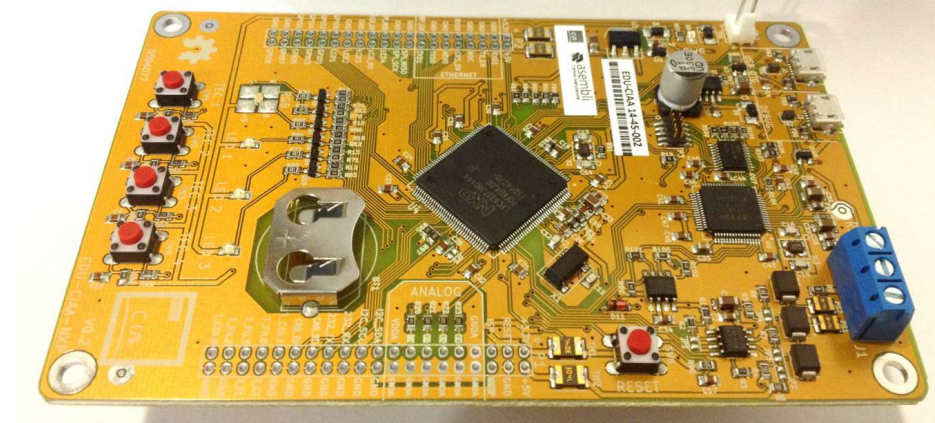
\includegraphics[width=10 cm]{figuras/descripcion1.png}
\caption{Placa EDU CIAA}
\label{Fig_placa}
\end{figure}
\end{center}


La placa EDU CIAA es la versión educativa de ésta, la cual se encuentra diseñada con el propósito de conseguir una plataforma base para el desarrollo de proyectos educativos, en este caso, se busca proporcionar las bases del desarrollo de códigos utilizando RTOS.


\begin{figure}[!h]
\centering
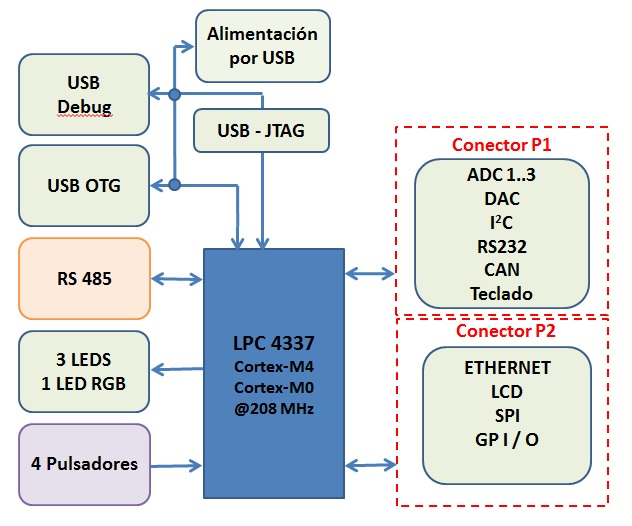
\includegraphics[width=8 cm]{figuras/diagramaenbloques.jpg}
\caption{Diagrama en bloques de EDU CIAA basado en LPC4337.}
\label{Fig1}
\end{figure}


El procesador que utiliza es el LPC4337, basado en el  ARM Cortex M4, utilizado para aplicaciones en sistemas embebidos, dicho sistemas incluyen el procesador Cortex M0. Utiliza una memoria flash de 1Mb, memoria de 264 kB de SRAM, memoria ROM de 64 kB, E2PROM de 16kB, y una memoria OTP de 64 bit.

La frecuencia de trabajo del procesador alcanza los 204 Mhz. Una característica vital del procesador, es que provee soporte para la depuración en JTAG, con posibilidad de incluir hasta 8 breakpoints, y 4 watchpoints.

Dicho procesador brinda una interface que hace posible extender hasta 164 pines de entrada-salida de propósito general (GPIO), provee una interface USB Host/Device 2.0 de alta velocidad con soporte para acceso directo de memoria, una interface UART 550 con soporte DMA , tres USART 550 con soporte para DMA\cite{descripcionenhojadatos}.

Como perifericos analógicos, debe destacarse la inclusión de un DAC de 10 bits, con soporte DMA y frecuencia de conversión de 400000 muestras por segundo. Dos ADC's con soporte DMA, y frecuencia de conversión de 400000 muestras por segundo, con un numero máximo de 8 canales sobre cada ADC. Y un ADC de 12 bits de 6 canales con soporte DMA, y frecuencia de conversión que puede alcanzar hasta los $80 . 10^6$ muestras por segundo.

El cristal oscilador posee un rango de operación desde 1 Mhz hasta 25 Mhz, este procesador incluye un reloj de tiempo real de baja potencia, el cual utiliza un oscilador de cristal.

La placa provee alimentación de 3,3 V (cuyo rango oscila entre 2,2 V hasta 3,6 V), y es capaz de operar en cuatro modos, los cuales se denominan \textit{sleep}, \textit{deep-sleep}, \textit{power-down},y \textit{deep power-down}.Es posible restablecer la operación de la placa desde los modos \textit{deep-sleep}, \textit{power-down}, y \textit{deep power-down}, a través de interrupciones externas.


\begin{figure}[!h]
\centering
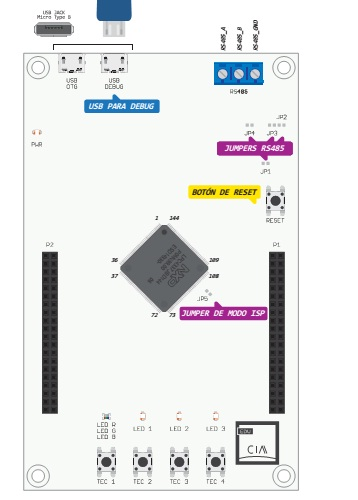
\includegraphics[width=6 cm]{figuras/FIGURA_1.jpg}
\caption{Imagen frontal de placa}
\label{Fig2}
\end{figure}

Sobre la Figura  \ref{Fig1} se proporciona el diagrama en bloques de la placa\cite{diagramaenbloquesdeplaca}, puede observarse que la placa cuenta con 2 puertos micro-USB (uno para aplicaciones y debugging, otro para alimentación); 4 salidas digitales implementadas con leds RGB, 4 entradas digitales con pulsadores; 1 puerto de comunicaciones RS485 con bornera. La Figura  \ref{Fig2} nos muestra  una imagen frontal de la placa; nótese la presencia de dos puertos sobre los cuales se ubican los pines correspondientes a la placa, la Figura  \ref{distribucionpines} ilustra el distribución de dichos pines sobre cada puerto.

Sobre el puerto P1, se ubican los siguientes módulos:

\begin{enumerate}
\item 3 entradas analógicas ($ADC0,1,2 y 3$)
\item 1 salida analógica (DAC0).
\item 1 puerto I2C.
\item 1 puerto asincrónico full duplex (para RS-232).
\item 1 puerto CAN.
\item 1 conexión para un teclado 3x4.
\end{enumerate}

Sobre el puerto P1, se ubican los siguientes módulos:

\begin{enumerate}
\item 1 puerto Ethernet
\item 1 puerto SPI
\item 1 puerto para Display LCD con 4 bits de datos, Enable y RS.
\item pines genéricos de I/0.
\end{enumerate}

\begin{figure}[h]
\centering
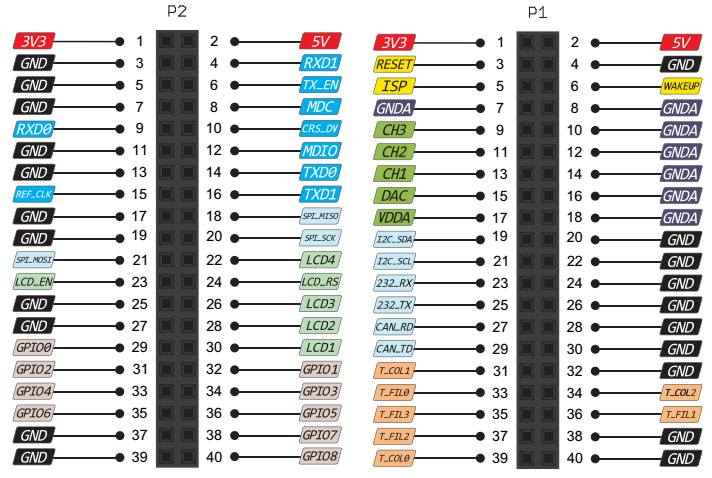
\includegraphics[width=8 cm]{figuras/f16.png}
\caption{Distribución de pines de la placa}
\label{distribucionpines}
\end{figure}

\section{Instalacion de Software}

\subsection{Conceptos previos}
El desarrollo de codigos para sistemas embebidos tiene ciertas semejanzas con el desarrollo de aplicaciones en las PC, en este caso particular se utiliza un compilador llamado \textit{GCC} con soporte para la compilación de proyectos sobre los procesadores basados en la arquitectura ARM. En este caso particular, el compilador utilizado para el procesador de la EDU CIAA (el LPC4337) se lo denomina \textit{arm-none-eabi-gcc}.

Para la ejecución de la depuración de algun programa previamente compilado, el hardware de la CIAA viene provisto con el chip \textit{FT2232H}, que se encarga de hacer un puente entre la interfase JTAG del microcontrolador, y el USB que conecta a la PC en el puerto USB dedicado al debug. Mediante la herramienta de código abierto \textit{OpenOCD (On Chip Debugger)} se controla el chip \textit{FT2232H} por el USB y ademas todo lo referido al JTAG. Luego la herramienta de depuración \textit{GDB} utilizado en el IDE-Eclipse que se instala, se comunica sobre el puerto 3333 (TCP) que el \textit{Open OCD} tiene en escucha esperando la conexión\cite{descripcionopenocd}.

Debe tenerse en cuenta que el chip \textit{FT2232H} posee 2 canales de comunicación independientes (A y B), sin embargo, ambos salen por el mismo USB, de modo que la PC detecta 2 dispositivos distintos (en realidad es uno compuesto). Uno de ellos, se conecta al JTAG manejado por \textit{OpenOCD} como fue mencionado, mientras que el otro se ve como un puerto virtual COM. Este último sirve principalmente para la depuración.
%%CONSIDERAR SI CIERTA PARTE VA A IR A SECCION INSTALACION

Dado que al funcionar como dos dispositivos distintos, para cada uno de ellos debe realizarse la instalación de un driver adecuado, en principio debe optarse por realizar la instalación de los drivers por defecto del fabricante FTDI para puerto virtual. %Considerar%

\subsection{Firmware de la EDU CIAA}
Considerando que el usuario previamente ha trabajado sobre placas de desarrollo tales como la MCE Debug, etc, y sobre microcontroladores PIC. Es necesario destacar un concepto teórico que brinda la posibilidad de fundamentar el trabajo sobre la placa EDU CIAA. Al trabajar sobre los otros dispositivos, es común la utilización de programas tales como \textit{MPLABX}, o \textit{PICC} a través del compilador \textit{CCS Compiler}; puntualmente; cuando se inicia un nuevo proyecto a traves de la herramienta de creación de la misma, es usual configurar este proyecto de manera que el software IDE genera un archivo \textit{makefile} para la compilación del proyecto.

En este caso, el software IDE de la EDU CIAA trabaja de forma ligeramente distinta, el usuario debe modificar un archivo \textit{makefile} (basándose en un archivo proporcionado previamente, denominado \textit{Makefile.config}) para poder efectuar la compilación del archivo y lograr la correcta configuración del programa, sobre la placa EDU CIAA. Dentro de él se establece la configuracion para la arquitectura del procesador utilizado.
%%CONSIDERAR POSICION DEL SIGUIENTE PARRAFO%%
Cuando se desea realizar el primer proyecto sobre la placa, el usuario debe crear su propio archivo \textit{Makefile.mine}, de manera que éste se encuentra basada en \textit{Makefile.config} brindado previamente al momento de establecer un nuevo proyecto añadiendo un Firmware que ha sido diseñado para el funcionamiento de la placa.

Debe tenerse en cuenta que la dinámica de trabajo sobre la placa se encuentra pensada para trabajar sobre la plataforma de versionado \textit{Git}; en este caso en particular, el archivo \textit{Makefile.mine} se encuentra diseñado de forma tal que dicho archivo sea ignorado al sincronizar su repositorio local, con su repositorio remoto (ubicado sobre \textit{Github}).

En \textit{Makefile.mine} se pueden editar y configurar los siguientes parámetros\cite{parametrosdelmakefile}:
\begin{enumerate}
\item \textbf{ARCH}  indica la arquitectura del hardware para la cual se desea compilar. Ej: x86, cortexM4.
\item \textbf{CPUTYPE} indica el tipo de CPU. Ej: none, ia32, ia64, lpc43xx.
\item \textbf{CPU} indica la CPU para la que se desea compilar. Ej: none, lpc4337.
\item \textbf{COMPILER }es el compilador a utilizar. Ej: gcc.
\item \textbf{BOARD }es la placa sobre la cual se trabajaca (CIAA-NXP, EDU-CIAA-NXP, etc.)
\item \textbf{PROJECT }es el Path al proyecto a compilar. Ej: examples$\$(DS)blinking_base$.
\end{enumerate}
Se utiliza la variable \$(DS) para indicar el separador de directorios (de manera automática se usa '/' para linux y \textbackslash{} para windows).

En el mismo Makefile aparecen al comienzo comentarios donde se indican los valores que pueden tomar estos parámetros.

Otro concepto importante que se tiene en cuenta cuando se desarrollan proyectos propios, es que cada proyecto tiene también su propio archivo \textit{Makefile}.El mismo se encuentra bajo el directorio \textbf{mak} en el directorio principal del proyecto o ejemplo. En el ejemplo \textbf{examples/blinking} el makefile del ejemplo se encuentra en \textbf{examples/blinking/mak} y se llama \textbf{Makefile}.

Sobre este archivo \textit{Makefile} contiene las siguientes definiciones:

\begin{enumerate}
\item \textbf{PROJECT} el nombre del proyecto y por ende nombre del ejecutable.
\item \textbf{\$(PROJECT)$\_$PATH} es el directorio del proyecto.
\item \textbf{INCLUDE} los paths a indicar al compilador para buscar includes files.
\item \textbf{SRC$\_$FILES} archivos a compilar ya sean archivos c como c++.
\item \textbf{OIL$\_$FILES} configuración del sistema operativo (si es utilizado).
\end{enumerate}

Cada proyecto incluye en su Makefile los módulos a compilar en una variable llamada MODS, por ejemplo:

MODS += modules$\$(DS)posix$ \  

        modules$\$(DS)ciaak $\  
        
        modules$\$(DS)config$ \  
        
        modules$\$(DS)bsp $\	
        
        modules$\$(DS)platforms$

Es recomendable utilizar \$(DS) en vez de / o \textbackslash{} para mantener la compatibilidad entre sistemas operativos (Linux, Windows, MAC OS).
{
\subsection{Estructura de Directorios de Firmware de EDU CIAA}
En el directorio principal luego de hacer un git clone o al bajar una release oficial se pueden encontrar los siguientes Directorios y Archivos\cite{estructuradedirectorios}:


\begin{figure}[!h]
\centering
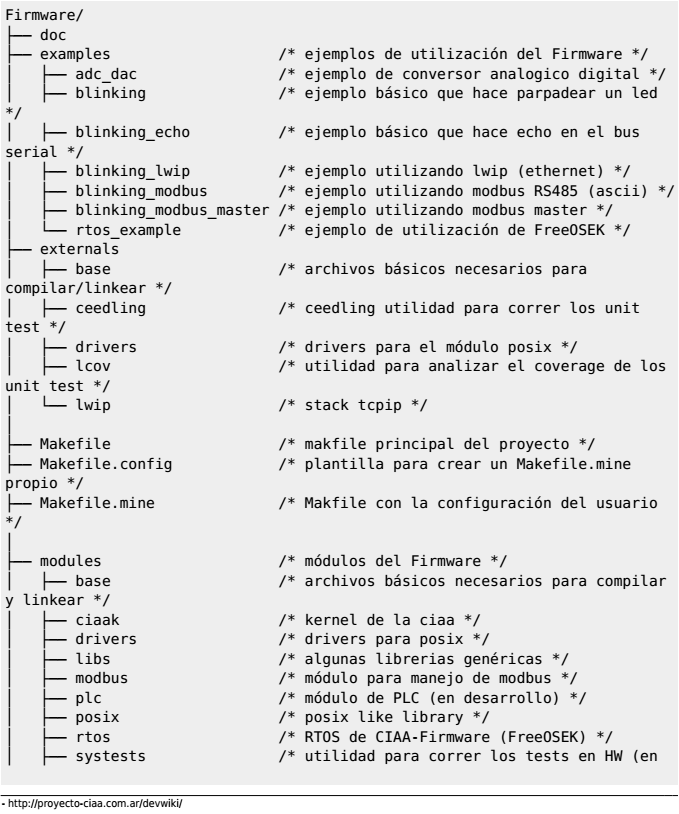
\includegraphics[width=8 cm]{figuras/est_directorios_ciaa.png}\\
\caption{Estructura de directorios del Firmware}
\label{Fig3}
\end{figure}

\textbf{Directorio $"externals"$(Software y Tools Externos)}\\
Este directorio contiene el Software y Tools externos al CIAA-Firmware, que son necesarios para compilar, testear, etc. el Firmware. Tenga en cuenta que el Software y Tools en esta carpeta no son parte de CIAA-Firmware y pueden contener otras licencias. Sobre el Cuadro \ref{Tab1} se ilustra los contenidos del directorio y su descripción. La Figura 3 ilustra los contenidos de la estructura de directorios.

\begin{table}
\begin{center}
\resizebox{18cm}{!}{
\begin{tabular}{|l|l|}
\hline\hline
ceedling & Tool utilizada para los Unit Tests o Pruebas Unitarias\\ \hline
base & Fuentes, headers y linker scripts necesarios para poder compilar y linkear el código en la plataforma\\ \hline
drivers & Drivers provistos por el proveedor del chip, los cuales son luego adaptados al formato de la CIAA.\\ \hline
\end{tabular}
}
\caption{Utilidades,archivos,y drivers para la placa}
\label{Tab1}
\end{center}
\end{table}

El Cuadro \ref{Tab2} contiene todos los archivos generados por el CIAA-Firmware:

\begin{table}[h]
\begin{center}
\resizebox{18cm}{!}{
\begin{tabular}{|l|l|}
\hline\hline
bin & Contiene el binario del proyecto, es el archivo que se va a correr en la PC o a cargar en el CIAA-Firmware\\ \hline
gen & Archivos generados de OSEK RTOS\\ \hline
lib & Por cada Módulo el make genera un archivo .a, osea una libreria\\ \hline
obj & Todos los archivos fuentes son compilados a object files y almacenados en este directorio\\ \hline
\end{tabular}
}
\caption{Descripción de archivos generados en un proyecto en RTOS.}
\label{Tab2}
\end{center}
\end{table}

}
\subsection{Iniciación a través de ejemplos}
En el Firmware de la placa se pueden varios ejemplos, estos se encuentran en la carpeta \textbf{examples} y pueden ser utilizados como base para iniciar cualquier proyecto.

Cualquiera de los ejemplos puede ser copiado y utilizado de base para nuevos proyectos. Por ejemplo con el siguiente comando:	\textit{cp -r $examples/blinking projects/my$\_$proyect$} y adaptando el Makefile.mine indicado: $PROJECT$\_$PATH = projects/my$\_$project$.
\subsection{Instalación de IDE}
El entorno de desarrollo integrado (IDE) posibilita el trabajo en un ambiente ameno, además provee las herramientas necesarias para el desarrollo de aplicaciones en el Firmware de forma automatica. La CIAA utiliza una version modificada de la plataforma de software (IDE)  \textit{Eclipse}, denominada \textit{CIAA-Software-IDE} ,la cual contiene herramientas de programación tales como editor de texto, compilador,plataforma para depuración, etc.
Sobre la página web del proyecto, se provee un instalador llamado \textit{CIAA-IDE-SUITE}, desde donde se puede configurar automáticamente todas las herramientas necesarias para trabajar con la placa. Este instalador solamente es para los usuarios que poseen Windows XP o superior.\\

El paquete de instalación incluye:
\begin{enumerate}
\item \textbf{Eclipse}
\item\textbf{PHP (Hypertext Pre-processor )} es un lenguaje de programación de uso general de código desde el lado del servidor, originalmente diseñado para el desarrollo de contenido dinámico. En este caso, se utiliza solamente en forma de scripts para poder generar algunos archivos del \textbf{Sistema Operativo OSEK}
\item \textbf{Cygwin} es una consola que se ejecuta en Windows, de modo de emular la consola de comandos de Linux. Cuenta con todos los comandos, y el compilador GCC, propio del sistema operativo libre.
\end{enumerate}

Una vez realizada la descarga del instalador, se ejecuta dicha aplicación, la figura \ref{Fig4} muestra el arranque del instalador, sobre ella, debe seleccionarse \textit{Siguiente}.A continuación deben aceptarse los términos de uso: 

\begin{figure}[!h]
\centering
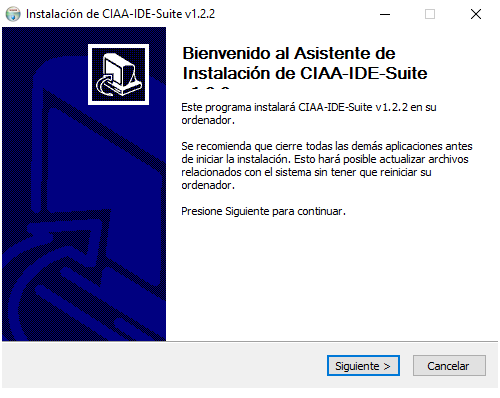
\includegraphics[width=8 cm]{figuras/instalacion1.png}\\
\caption{Arranque del instalador del software IDE}
\label{Fig4}
\end{figure}

\begin{figure}[!h]
\centering
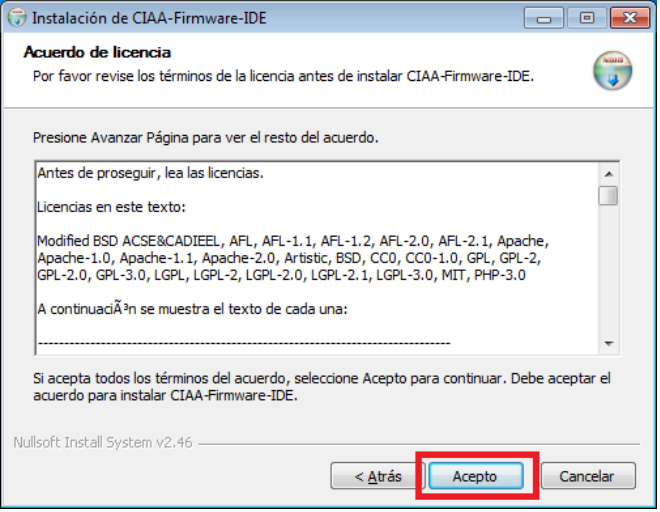
\includegraphics[width=8 cm]{figuras/instalacion2.png}\\
\caption{Arranque del instalador del software IDE}
\label{Fig5}
\end{figure}

Sobre la ventana siguiente deben elegirse cuáles componentes se desea instalar, en el caso que el usuario no posea  la placa disponible, no es necesario instalar los drivers, si se adquiere dicha placa en un momento posterior,dado que los drivers se instalan junto con el IDE, los mismos quedarán en la carpeta de destino para su instalación en forma manual; otra forma de instalar los  los controladores es ejecutar el instalador del CIAA-IDE Suite y tildar únicamente la opción \textbf{drivers} al momento de seleccionar los componentes a instalar.La Figura \ref{Fig5} ilustra lo explicado anteriormente. Sobre la Figura \ref{Fig6}, se deben seleccionar los componentes a instalar.

\begin{figure}[!h]
\centering
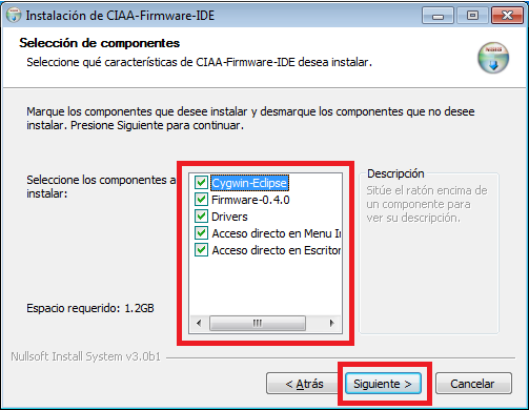
\includegraphics[width=8 cm]{figuras/instalacion3.png}\\
\caption{Selección de componentes del instalador}
\label{Fig6}
\end{figure}

\begin{figure}[!h]
\centering
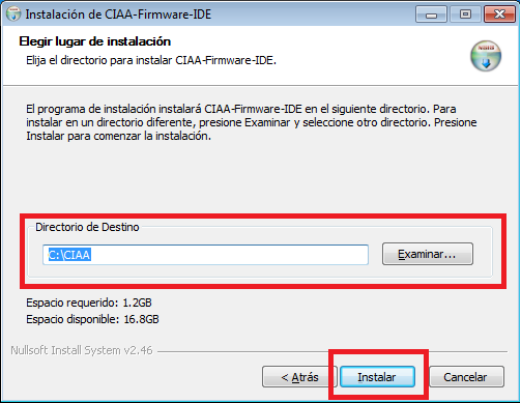
\includegraphics[width=8 cm]{figuras/instalacion4.png}\\
\caption{Elección de la ruta de instalación}
\label{Fig7}
\end{figure}

A continuación debe  establecerse la dirección en donde se desea instalar el entorno. La ventana que corresponde a este proceso se ilustra en la Figura \ref{Fig7}. En caso de que se desee cambiar dicha dirección,debe tenerse la precaución de no elegir una dirección donde los directorios posean espacios en sus nombres. Es recomendable no cambiar la unidad de instalación, pues en los siguientes pasos del documento se utilizarán direcciones que harán referencia a esta carpeta de instalación, y si se cambia, se deberán cambiar consecuentemente dichas direcciones.

Luego de dicha configuración, se inicia automáticamente el proceso de instalación.En un momento aparecerá una ventana emergente, similar a la que se muestra en la Figura \ref{Fig8}, en donde el programa pregunta si se dispone del hardware, pues para la instalación del driver es necesario conectar la placa. De no  ser así, aún puede continuar la instalación haciendo click en 'No'. Por el contrario, si se dispone de la EDU-CIAA, se debe hacer click en 'Yes', y emergerá otra ventana, como se muestra en la Figura \ref{Fig9}.

\begin{center}
\begin{figure}[!h]
\centering
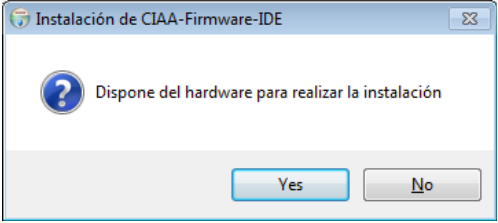
\includegraphics[width=6 cm]{figuras/instalacion5.png}\\
\caption{Instalación de los drivers: primera instancia}
\label{Fig8}
\end{figure}
\end{center}


\begin{figure}[!h]
\centering
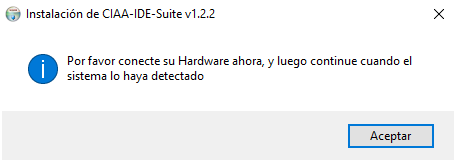
\includegraphics[width=6 cm]{figuras/instalacion6.png}\\
\caption{Instalación de drivers si se dispone del hardware}
\label{Fig9}
\end{figure}

Una vez finalizada esta etapa, se procede a la instalación de los drivers por defecto del fabricante FTDI para puerto virtual. Este proceso se ilustra en las figuras \ref{driversFTDI} ,\ref{Fig10},\ref{Fig11},\ref{Fig12} y \ref{Fig13}.
\begin{center}
\begin{figure}[!h]
\centering
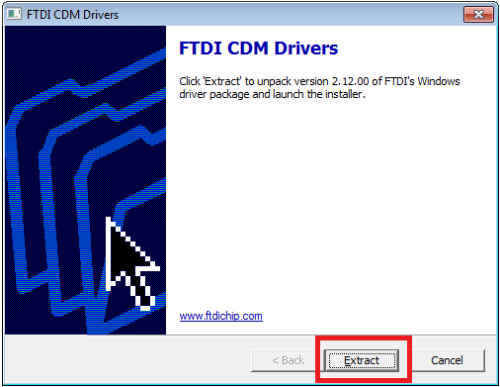
\includegraphics[width=6 cm]{figuras/instalacion7.png}\\
\caption{Instalador de drivers FTDI parte 1}
\label{driversFTDI}
\end{figure}
\end{center}
\begin{center}
\begin{figure}[!h]
\centering
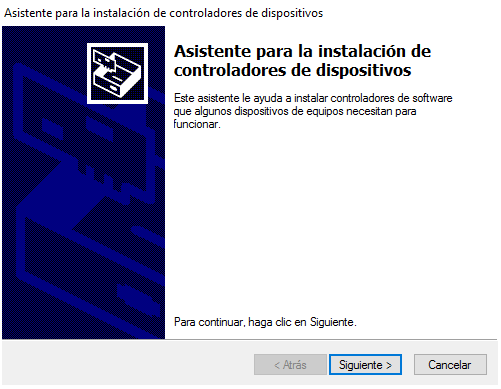
\includegraphics[width=5 cm]{figuras/instalacion8.png}\\
\caption{Instalador de drivers FTDI parte 2}
\label{Fig10}
\end{figure}
\end{center}
\begin{center}
\begin{figure}[!h]
\centering
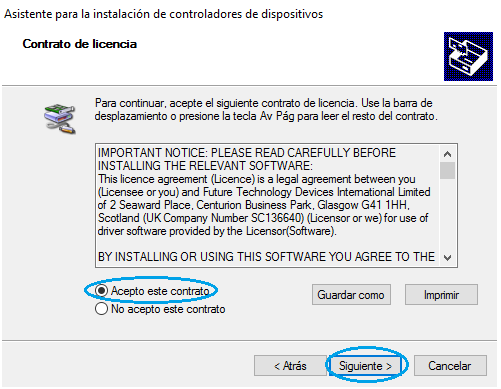
\includegraphics[width=6 cm]{figuras/instalacion9.png}\\
\caption{Instalador de drivers FTDI parte 3}
\label{Fig11}
\end{figure}
\end{center}
\begin{center}
\begin{figure}[!h]
\centering
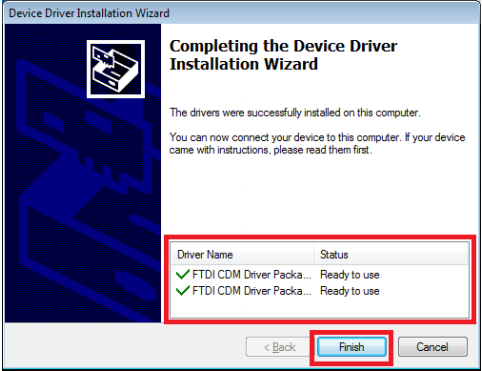
\includegraphics[width=6 cm]{figuras/instalacion10.png}\\
\caption{Instalador de drivers FTDI parte 4}
\label{Fig12}
\end{figure}
\end{center}
\begin{figure}[!h]
\centering
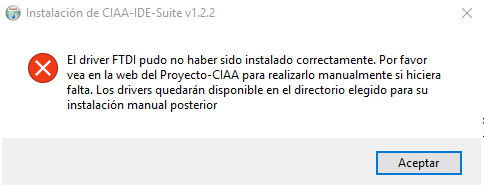
\includegraphics[width=9 cm]{figuras/instalacion11.png}\\
\caption{Instalador de drivers FTDI parte 5}
\label{Fig13}
\end{figure}
Una de las posibles fallas que pueden surgir a través de este proceso, se presenta al producirse una falla en la comunicación a través del puerto virtual FTDI, que impide la correcta comunicación entre la placa y el entorno IDE. Su corrección debe efectuarse manualmente, fuera del instalador, y es posible la aparición de una ventana de error emergente como la que se muestra en la Figura \ref{Fig13}.

El instalador incluye en la carpeta donde se instaló el software (Por defecto, $ C:/CIAA $ ) un programa que configura el driver del controlador serie,emulado por la placa, para que uno de ellos pueda ser utilizado como interfaz JTAG. Dicho programa se llama $ Zadig\_Win\_7\_2\_1\_1.exe $, la Figura \ref{Fig14} muestra una ilustración de la ubicación del programa.

\begin{figure}[!h]
\centering
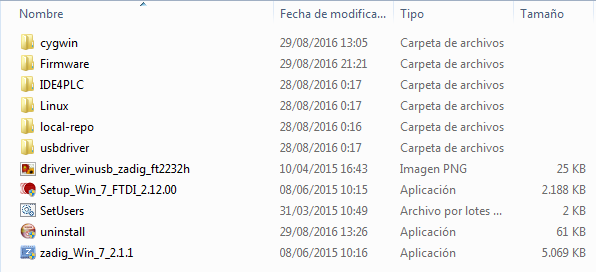
\includegraphics[width=6 cm]{figuras/instalacion12.png}\\
\caption{Instalador de drivers FTDI parte 6}
\label{Fig14}
\end{figure}
Al abrir la aplicación, se presenta la Figura \ref{Fig15}. Antes de proceder, el usuario debe conectar la placa, posteriormente, debe abrir el menú contextual \textit{Options} y presionar sobre \textit{List all devices}

\begin{figure}[!h]
\centering
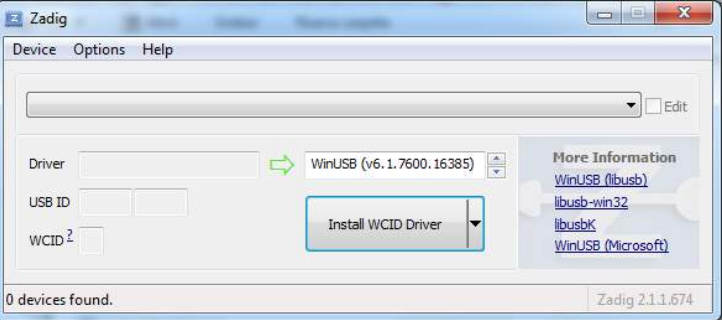
\includegraphics[width=6 cm]{figuras/instalacion13.png}\\
\caption{Entorno del software corrector Zadig para Windows}
\label{Fig15}
\end{figure}
Aparecerá una lista de dispositivos de comunicación relacionados al USB. Se tiene que buscar aquellos cuyos nombres tengan relación con el puerto serie (puede aparecer Dual RS232-HS, USB Serial Converter, o algo similar).

Por lo general, aparecerán 2 con el mismo nombre, excepto que uno es Interface 0 y el otro Interface 1, como se muestra en la Figura \ref{Fig16} (la lista de drivers que se muestra puede diferir, dependiendo de la computadora que se utilice).

\begin{figure}[!h]
\centering
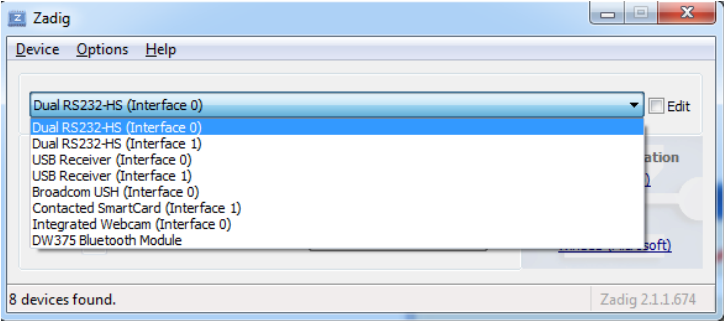
\includegraphics[width=8 cm]{figuras/instalacion14.png}\\
\caption{Lista de dispositivos vinculados a USB}
\label{Fig16}
\end{figure}
Para configurar el driver:

\begin{enumerate}
\item[1]seleccionar la \textbf{Interfase 0}
\item[2]elegir el \textbf{“WinUSB v6.1”}
\item[2]hacer click en el botón \textbf{“Replace Driver”}.
\end{enumerate}

La Figura \ref{Fig17} muestra la ventana ya configurada:


\begin{figure}[!h]
\centering
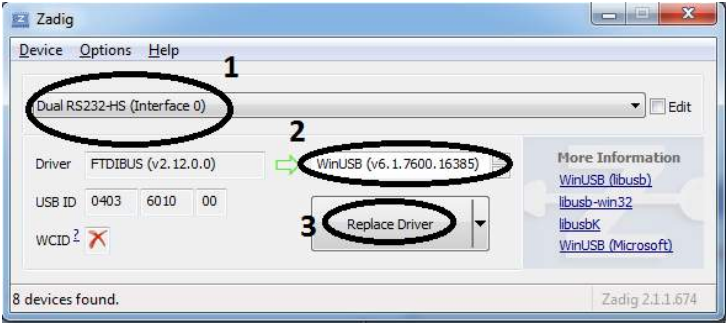
\includegraphics[width=8 cm]{figuras/instalacion15.png}\\
\caption{Configuración del Zadig para el reemplazo del driver}
\label{Fig17}
\end{figure}


\section{Desinstalación}
Si se instaló el Software de CIAA-IDE y luego se desea desinstalarlo, se debe tener especial
cuidado en quitar cualquier contenido que se quiera conservar de la carpeta $C:\_\ CIAA$, o el
directorio de instalación elegido. Esto se debe a que el desinstalador del Software CIAA-IDE
elimina el directorio y todo su contenido.

\section{Primeros Pasos con la EDU-CIAA}

\subsection{Programacion en Baremetal a través de libreria sAPI}\label{programacionbaremetal}
Debido a que la programación de la placa en Baremetal puede tornarse un tanto engorrosa en principio, es posible utilizar una libreria diseñada para la implementación de proyectos en Baremetal con la placa EDU CIAA, dicha librería se la denomina \textit{sAPI}. Esta biblioteca implementa una API simple para la programación de dicha placa, es necesario comentar que una API es una interfaz de programación de aplicaciones, y consta de un conjunto de subrutinas, funciones y procedimientos (o métodos, en la programación orientada a objetos) que ofrece cierta biblioteca; para permitir ser utilizada por otro software como una capa de abstracción en la programación (aunque no necesariamente) entre los niveles o capas inferiores y las superiores del software\cite{sapi}.

La motivación para el desarrollo de la biblioteca sAPI surge de la necesidad de manejar los periféricos directamente desde una máquina virtual de Java para el desarrollo de Java sobre la CIAA y corresponde a la parte de bajo nivel de las clases de periféricos en Java que básicamente bindea a funciones escritas en C.
Luego se extendió la misma para facilitar el uso de la EDU-CIAA-NXP a personas no expertas en la arquitectura del LPC4337 facilitando el uso de esta plataforma.

La idea es tener periféricos abstractos y lo más genéricos posibles. Que sea bien independiente de la arquitectura y en lo posible que las funciones sean todas del tipo:
\begin{enumerate}
\item[$\bullet$]	moduloConfig();
\item[$\bullet$]  moduloRead();
\item[$\bullet$]  moduloWrite();
\end{enumerate}
Los siguientes módulos estan incluidos:
\begin{enumerate}
\item[$\bullet$]Tipos de datos.
\item[$\bullet$]Mapa de periféricos.
\item[$\bullet$]Plataforma.
\item[$\bullet$]Tick.
\item[$\bullet$]Retardo.
\item[$\bullet$]E/S Digital.
\item[$\bullet$]E/S Analógica.
\item[$\bullet$]Uart.
\end{enumerate}
 Es necesario destacar que actualmente se encuentra disponible para las plataformas EDU CIAA NXP (microcontrolador NXP LPC4337) y para la plataforma CIAA NXP (microcontrolador NXP LPC4337). La Figura \ref{Fig18} ilustra como son las distintas capas de software y la correspondiente ubicación de la \textit{sAPI}.\\
\underline{Breve descripcion de los modulos de la biblioteca}:
\begin{enumerate}
\item[•]\textbf{sAPI$\_$Config}: Contiene configuraciones de la biblioteca.
\item[•]\textbf{sAPI$\_$DataTypes}:Define las siguientes constantes:
\begin{enumerate}
\item[•]Estados lógicos, \textit{TRUE} y \textit{FALSE}.
\item[•]Estados funcionales \textit{ON} y \textit{OFF}
\item[•]Estados electricos \textit{HIGH} y \textit{LOW}
\item[•]Tipos de datos: Booleanos (\textit{bool$\_$t}), enteros sin signo(\textit{uint8$\_$t, uint16$\_$t, uint32$\_$t, uint64$\_$t}), enteros con signo (\textit{int8$\_$t, int16$\_$t, int32$\_$t, int64$\_$t}).
\end{enumerate}
\item[•]\textbf{sAPI$\_$IsrVector}:Contiene la tabla de vectores de interrupción.
\item[•]\textbf{sAPI$\_$Board}:Contiene la función de configuración para inicialización de la plataforma de hardware.
\item[•]\textbf{sAPI$\_$PeripheralMap}:Contiene el mapa de periféricos, para la interpretación de éste, el usuario debe utilizar el diagrama esquemático de la placa y el archivo \textit{PeripheralMap$.txt$} ubicado sobre el directorio \textit{sapi-bm}.
\item[•]\textbf{sAPI$\_$DigitalIO}: Utilizada para el manejo de entradas y salidas digitales.
\end{enumerate}
 
\begin{figure}[!h]
\centering
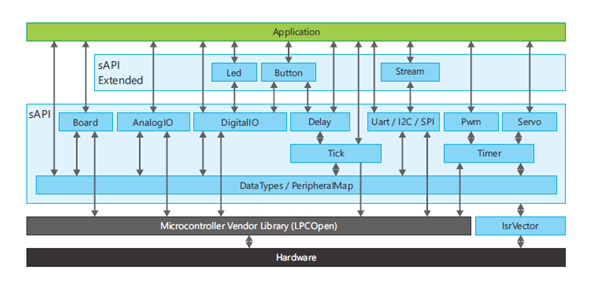
\includegraphics[width=12 cm]{figuras/primer_proy18.png}\\
\caption{Capas de abstracción de software}
\label{Fig18}
\end{figure}

\underline{Utilización de librería sAPI}:

Es posible descargar la version más reciente de dicha biblioteca, a traves del repositorio de la misma, ubicado en la pagina web (especificar la referencia a la pagina web del repositorio).

Luego de haber descargado la versión actual de  sAPI se procede a copiar la carpeta \textit{sapi$\_$bm} y pegarla en \textit{C$:/$CIAA$/$Firmware$/$modules}.

A continuación, el usuario debe crear un directorio el cual contiene al proyecto, y sobre el mismo, deben realizarse los directorios que contengan las cabeceras, el \textit{Makefile}, y los archivos fuentes.

Al utilizar la biblioteca \textit{sAPI} para un proyecto en Baremetal, se debe modificar el makefile del mismo dentro de la carpeta mak y cambiar la última línea de: \textbf{MODS += externals \$(DS)drivers}, y reemplazarla por:  \textbf{MODS += modules \$ (DS)sapi$\_$bm}.

Luego, sobre cada archivo fuente en la que se ejecuten instrucciones que contenga esta librería, se debe realizar la inclusión del mismo mediante la instruccion: \textbf{\# include “sAPI.h”}. Debe aclararse que en la versión 0.3.0 no es necesario incluir el archivo \textit{chip.h} dado que la propia biblioteca lo incluye, además, esta librería maneja el vector de interrupción, por lo tanto, para el usuario que haya trabajado anteriormente con proyectos escritos en instrucciones de \textit{LPCOpen}, debe tenerse en cuenta que ya no se necesita realizar el archivo que contenga las direcciones de las subrutinas para la atención de las interrupciones. El ejemplo \textit{"baremetal"} del Firmware en el que se realiza este tutorial, trae consigo dicho archivo.

Es importante tener en cuenta que para la compilación y depuración del programa mediante el IDE del Firmware, se debe colocar sobre la carpeta Firmware y mediante click derecho, el usuario debe ubicarse en \textit{Propiedades}$\rightarrow$\textit{C/C++ Build}$\rightarrow$\textit{Behaviour}. A continuación debe modificar sobre la rama \textit{Clean}, y reemplazar la palabra \textit{Clean\_ generate} por la palabra \textit{clean}, como puede apreciarse en la Figura \ref{Fig19}.
\begin{center}
\begin{figure}[!h]
\centering
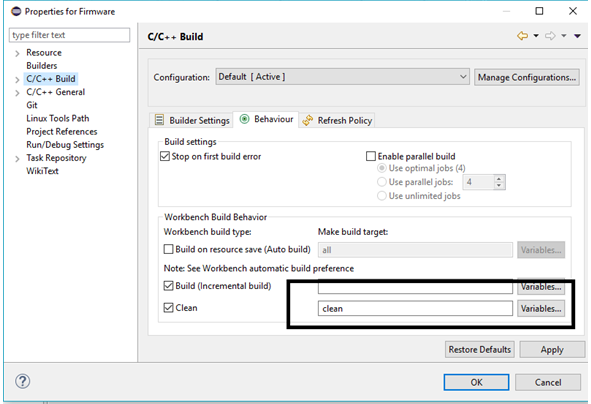
\includegraphics[width=8 cm]{figuras/f1.png}\\
\caption{Cambio de “clean\_ generate” a “clean”.}
\label{Fig19}
\end{figure}
\end{center} 
\subsubsection{Implementacion de ejemplo N$^{\circ}$1: Salidas Digitales}
El primer ejemplo aborda las salidas digitales, a través de los leds que provee la placa EDU-CIAA.

Este programa enciende los leds de la placa en forma secuencial, de izquierda a la derecha. Luego de finalizar esta secuencia, se apagan de derecha a izquierda.

Debe destacarse que sobre el inicio del programa fuente se realizan las inclusiones de el archivo cabecera del proyecto y la biblioteca \textit{sAPI}.La Figura \ref{Fig20} ilustra lo explicado anteriormente.

\begin{center}
\begin{figure}[!h]
\centering
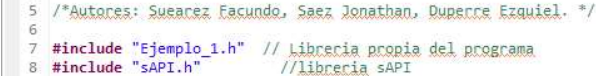
\includegraphics[width=6 cm]{figuras/f2.png}\\
\caption{Inclusión de archivo cabecera y libreria}
\label{Fig20}
\end{figure}
\end{center}
	
Sobre el código del programa, es importante destacar algunas funciones utilizadas:

\begin{enumerate}
\item[•]\textbf{Boardconfig()}: Esta función se encarga de la configuración para inicializar la plataforma del hardware.
\item[•]\textbf{Tickconfig()}:Configura una interrupción periódica de temporizador cada tickRateMSvalue milisegundos para utilizar de base de tiempo del sistema.El primer parámetro es el tiempo en milisegundos en el que se desee interrumpir el perifèrico Systick y aumente un contador que se usa para
el mòdulo delay o para lo que se requiera. 
\item[•]\textbf{Digitalconfig()}: Configuración inicial y modo de una entrada o salida.
\item[•]\textbf{DigitalWrite()}:Esta función se encarga de la escritura de salida digital, en este caso encienden los leds.
\item[•]\textbf{Delay()}:Esta función  realiza los retardos (con excepción del retardo inexacto) siempre y cuando peviamente se haya configurado el tick en el codigo.
\end{enumerate}
Para la compilación de dicho proyecto, debe tenerse en cuenta lo mencionado sobre la seccion \ref{sec:programacionbaremetal}, mientras que para implementar la depuración sobre la placa, el usuario debe seleccionar el archivo \textit{axf} que resulta de la compilación del proyecto.La Figura \ref{Fig21} ilustra la ventana resultante para la carga del programa.Este procedimiento, se repite para la implementación de todos los ejemplos. 

\begin{center}
\begin{figure}[!h]
\centering
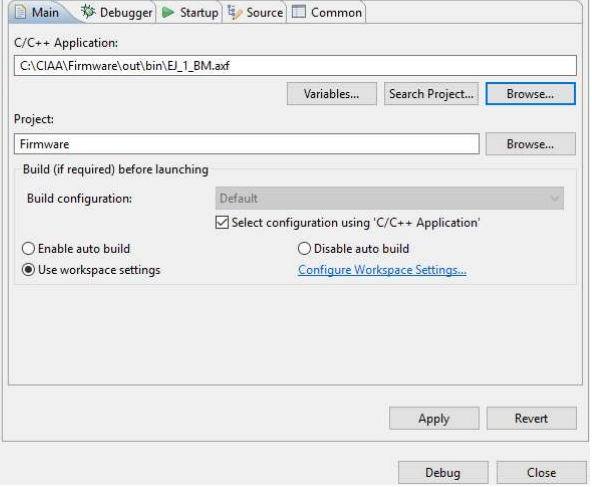
\includegraphics[width=6 cm]{figuras/f3.png}\\
\caption{Inclusión de archivo cabecera y libreria}
\label{Fig21}
\end{figure}
\end{center}
\subsubsection{Implementacion de ejemplo N$^{\circ}$2: Entradas y Salidas Digitales}\label{sec:ej2BM}

El siguiente ejemplo tiene como objetivo el manejo de las entradas y salidas digitales, dicho programa enciende los leds instalados sobre la placa, de acuerdo con la cantidad de veces que se oprime la tecla \textit{TEC1}. Sobre dicho ejemplo se implemento una maquina de estado, a través del programa \textit{uModel Factory} para poder establecer un orden sobre los eventos y las acciones que debe ejecutar el procesador. Debe tenerse en cuenta que se implementan multiples archivos fuentes y cabeceras, en particular, el archivo fuente \textit{FUNC$\_$EJ2$\_$BM.c} define las acciones y la evaluación de los eventos y \textit{FUNC$\_$EJ2$\_$BM.h} establece la declaración de dichas funciones y de los estados.

La funcion \textit{digitalRead} se encarga de las entradas digitales. En este caso se pregunta  si se ha oprimido la tecla 1, como se puede apreciar esta misma se activa por bajo, por eso se pregunta si la lectura es igual a OFF.

A continuación se realiza una breve descripción de los estados, eventos y acciones que contiene este programa.
\begin{enumerate}
\item[•]\underline{Estados}:
\begin{enumerate}
\item[•]Estado \textit{\textbf{INICIAL}}: Estado inicial en el cual, si se oprime la tecla \textit{TEC1}, se ejecuta la acción \textit{LED$\_$R}.
\item[•]Estado \textit{\textbf{ROJO}}: El codigo establece que al oprimir la tecla \textit{TEC1}, se ejecuta la acción \textit{P$\_$LED1}. 
\item[•]Estado \textit{\textbf{LED$\_$1}}: El codigo establece que al oprimir la tecla \textit{TEC1}, se ejecuta la acción \textit{P$\_$LED2}.
\item[•]Estado \textit{\textbf{LED$\_$2}}: El codigo establece que al oprimir la tecla \textit{TEC1}, se ejecuta la acción \textit{P$\_$LED3}.
\item[•]Estado \textit{\textbf{LED$\_$3}}: El codigo establece que al oprimir la tecla \textit{TEC1}, se ejecuta la acción \textit{P$\_$LED3}.  
\end{enumerate}
\item[•]\underline{Eventos}:
\begin{enumerate}
\item[•]Evento \textit{\textbf{PRESIONO}}: Identifica si se oprime la tecla \textit{TEC1}.
\item[•]Evento \textit{\textbf{PRESIONO$\_$4}}: Identifica si se oprime la tecla \textit{TEC1} en la primer secuencia.
\item[•]Evento \textit{\textbf{PRESIONO$\_$7}}: Identifica si se oprime la tecla \textit{TEC1} en la segunda secuencia.
\item[•]Evento \textit{\textbf{PRESIONO$\_$10}}: Identifica si se oprime la tecla \textit{TEC1} en la tercer y ultima secuencia.
\end{enumerate}
\item[•]\underline{Acciones}:
\begin{enumerate}
\item[•]Accion \textit{\textbf{LED$\_$R}}: Encendido de \textit{LEDR},\textit{LEDB},\textit{LEDG} según corresponda.
\item[•]Accion \textit{\textbf{P$\_$LED$\_$1}}: Encendido de \textit{LED1}.
\item[•]Accion \textit{\textbf{P$\_$LED$\_$2}}: Encendido de \textit{LED2}.
\item[•]Accion \textit{\textbf{P$\_$LED$\_$3}}: Encendido de \textit{LED3}.
\end{enumerate}
\end{enumerate}

La Figura \ref{Fig22} especifica el diagrama de estados del ejemplo:
\begin{center}
\begin{figure}[!h]
\centering
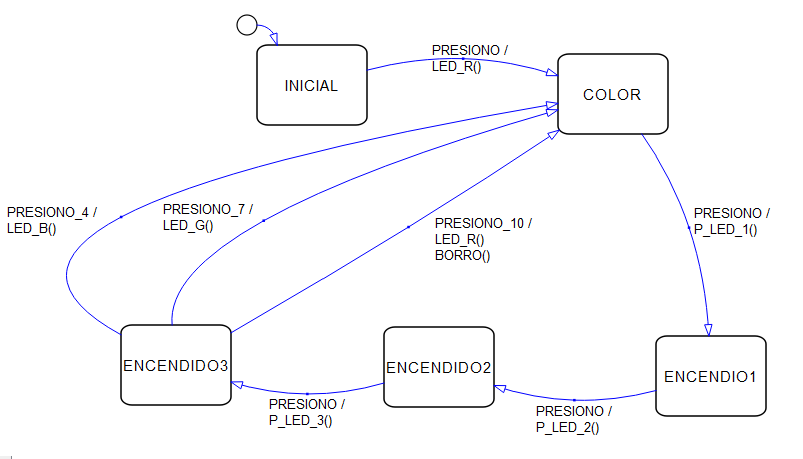
\includegraphics[width=7 cm]{figuras/f4.png}\\
\caption{Diagrama de estados de ejemplo N$^{\circ}$2}
\label{Fig22}
\end{figure}
\end{center}
\subsubsection{Implementacion de ejemplo N$^{\circ}$3: Entradas Analógicas y Uso de Display 7 segmentos}
En este ejemplo se realizan dos tareas distintas, dependiendo de la tecla pulsada (\textit{TEC1} y \textit{TEC2}).Si se pulsa la tecla \textit{TEC1}, se encienden los Leds en una secuencia determinada. Mientras que si se pulsa la tecla \textit{TEC2}, se realiza una muestra de los dígitos desde 1 hasta 9 a través del display 7 segmentos. 

Se implementa una maquina de estados en donde se establecen los prototipos de funciones que corresponden a los eventos y las acciones que acontecen. 

Para el manejo del display se utiliza una biblioteca. Para ello, deben generarse dos archivos los cuales pertenecen a la cabecera y a la fuente de dicha biblioteca. Sobre la cabecera deben establecerse las inclusiones de la biblioteca \textit{sAPI} y las declaraciones de las funciones que corresponden con el manejo del dispositivo.

En este tutorial se realiza el manejo de un display de 7 segmentos del tipo cátodo común, de manera que para provocar el encendido de un led perteneciente al arreglo, se debe establecer en alto la salida de el pin conectado a dicho led. La biblioteca que provee este tutorial determina el conexionado de los pines del display, sobre los correspondientes terminales GPIO ubicados en la placa EDU CIAA. La Figura \ref{Fig23} ilustra los terminales de la placa y del display utilizados para la conexión del dispositivo.

\begin{center}
\begin{figure}[!h]
\centering
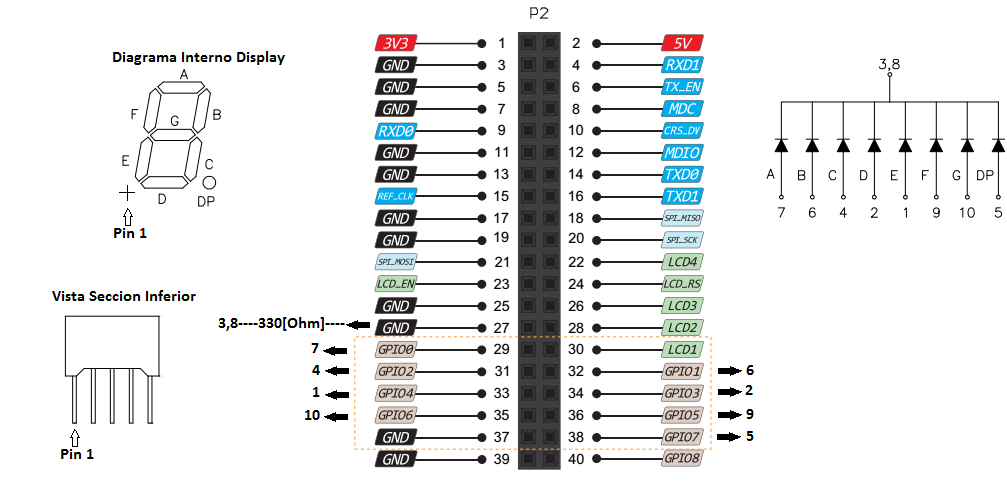
\includegraphics[width=10 cm]{figuras/f5.png}\\
\caption{Diagrama de conexión display 7 segmentos.}
\label{Fig23}
\end{figure}
\end{center}

A continuación se realiza una breve descripción de los estados, eventos y acciones que contiene este programa.
\begin{enumerate}
\item[•]\underline{Estados}:
\begin{enumerate}
\item[•]Estado \textit{\textbf{INICIAL}}: Estado inicial en el cual, en presencia del evento \textit{NO$\_$APRETO}, el programa se establece en el mismo estado; mientras que para el caso que suceda evento \textit{APRETO1}, el programa se establece en el estado \textit{ESTADO1}; en el caso de la ocurrencia del evento \textit{APRETO2}, el programa se establece en el estado \textit{ESTADO2}. 
\item[•]Estado \textit{\textbf{ESTADO1}}: Sobre dicho estado se realiza la secuencia de luces y la muestra de los digitos decimales sobre el display.
\item[•]Estado \textit{\textbf{ESTADO2}}: Sobre dicho estado se muestra de un digito decimal en caso de que se oprima la tecla \textit{TEC2}.
\end{enumerate}
\item[•]\underline{Eventos}:
\begin{enumerate}
\item[•]Evento \textit{\textbf{NO$\_$APRETO}}: Identifica si no se ha oprimido la tecla \textit{TEC1} o la tecla \textit{TEC2}.
\item[•]Evento \textit{\textbf{APRETO1}}: Identifica si se oprime la tecla \textit{TEC1}.
\item[•]Evento \textit{\textbf{APRETO2}}: Identifica si se oprime la tecla \textit{TEC2}.
\end{enumerate}
\end{enumerate}
La Figura \ref{Fig27}, ilustra el diagrama de estados de este ejemplo:

\begin{center}
\begin{figure}[!h]
\centering
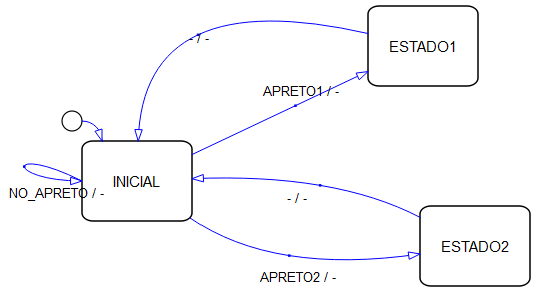
\includegraphics[width=6 cm]{figuras/f9.png}\\
\caption{Diagrama de estados de ejemplo N$^{\circ}$3.}
\label{Fig27}
\end{figure}
\end{center}
\underline{Uso de Entradas Analógicas}:

En este código se hará uso del conversor analógico digital que posee esta placa. La idea es introducir una tensión analógica mediante la entrada CH1 y luego convertirla en un valor digital, para que posteriormente dentro del código, mediante operaciones matemáticas, poder mostrar dicho valor por el display.
En la figura 5.4 se muestra un extracto del código principal donde se hace uso del ADC. Como se ver en esta figura, se utiliza la función analogRead (AIO), la cual se encarga de tomar el valor de tensión ingresado por la entrada analógica y convertirla a un valor digital. 

\subsubsection{Implementacion de ejemplo N$^{\circ}$4: Conversor Digital/Analógico (DAC)}

Un convertidor Digital/Analógico (DAC), es un dispositivo electrónico que recibe como dato de entrada un valor digital (en forma de una palabra de "n" bits) y lo transforma a una señal analógica. Cada una de las combinaciones binarias de entrada es convertida en niveles lógicos de tensión de salida. Un DAC transfiere información expresada en forma digital a una forma analógica. Para ubicar la función de este dispositivo conviene recordar que un sistema combina y relaciona diversos subsistemas que trabajan diferentes tipos de información analógica, como son; magnitudes eléctricas, mecánicas, etc.

El siguiente ejemplo muestra al usuario como realizar el uso del módulo ADC de la placa, para realizar la lectura de una entrada analógica. Este programa enciende algunos de los leds de la placa, en función a la magnitud de la tensión leída. Por ejemplo, si la tensión leída es 2[V], entonces se encienden dos leds.

La placa EDU-CIAA posee un DAC de 10 bits de resolución ,por lo tanto,el número de niveles de voltaje de salida analógico que es capaz de generar es de $2^{n}=2^{10}=1024$.

\begin{figure}[!h]
\centering
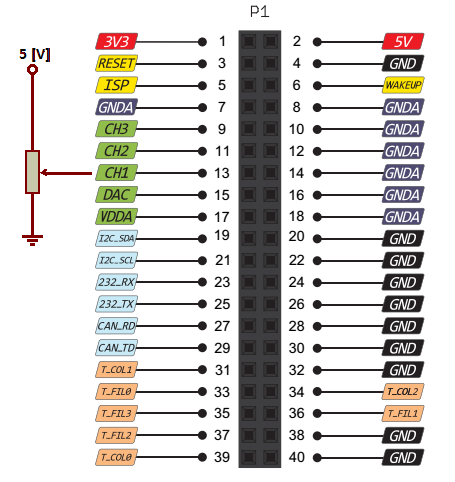
\includegraphics[width=6 cm]{figuras/f6.png}\\
\caption{Diagrama de conexión potenciómetro para lectura analógica.}
\label{Fig24}
\end{figure}

Para la implementación del ejemplo, es posible realizar la lectura del terminal medio de un potenciómetro, la Figura \ref{Fig24} ilustra la conexión realizada.Debe tenerse en cuenta que es posible realizar la conexión del potenciómetro a partir de la terminal de 5[V] y la terminal GNDA que ofrece la placa.

Este ejemplo utiliza maquinas de estado para poder establecer un orden sobre los eventos y las acciones que debe ejecutar el procesador.La Figura \ref{Fig25} especifica el diagrama de estados del ejemplo. A continuación se realiza una breve descripción de los estados, eventos y acciones que contiene este programa.

La instrucción \textit{analogConfig( ENABLE$\_$ANALOG$\_$INPUTS )} se encarga de habilitar las entradas analógicas. Mientras que \textit{analogConfig( ENABLE$\_$ANALOG$\_$OUTPUTS )} se encarga de habilitar las salidas analógicas, con las que trabajara el DAC.

\begin{center}
\begin{figure}[!h]
\centering
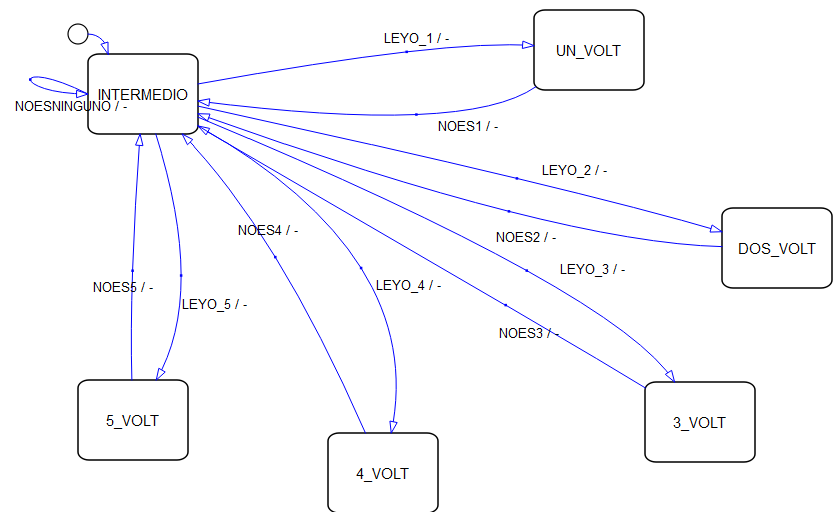
\includegraphics[width=10 cm]{figuras/f7.png}\\
\caption{Diagrama de estados de ejemplo N$^{\circ}$4.}
\label{Fig25}
\end{figure}
\end{center}


\begin{enumerate}
\item[•]\underline{Estados}:
\begin{enumerate}
\item[•]Estado \textit{\textbf{UN$\_$VOLT}}: Estado en el cual, la tensión leída es igual a 1[V].
\item[•]Estado \textit{\textbf{DOS$\_$VOLT}}: Estado en el cual, la tensión leída es igual a 2[V].
\item[•]Estado \textit{\textbf{TRES$\_$VOLT}}: Estado en el cual, la tensión leída es igual a 3[V].
\item[•]Estado \textit{\textbf{CUATRO$\_$VOLT}}: Estado en el cual, la tensión leída es igual a 4[V].
\item[•]Estado \textit{\textbf{INTERMEDIO}}: Estado inicial en el cual, la tensión leída no es igual a 1[V],2[V],3[V],4[V],o 5[V].
\end{enumerate}
\item[•]\underline{Eventos}:
\begin{enumerate}
\item[•]Evento \textit{\textbf{LEYO$\_$1}}: Identifica si la lectura realizada sobre el ADC corresponde a 1[V].
\item[•]Evento \textit{\textbf{LEYO$\_$2}}: Identifica si la lectura realizada sobre el ADC corresponde a 2[V].
\item[•]Evento \textit{\textbf{LEYO$\_$3}}: Identifica si la lectura realizada sobre el ADC corresponde a 3[V].
\item[•]Evento \textit{\textbf{LEYO$\_$4}}: Identifica si la lectura realizada sobre el ADC corresponde a 4[V].
\item[•]Evento \textit{\textbf{LEYO$\_$5}}: Identifica si la lectura realizada sobre el ADC corresponde a 5[V].
\item[•]Evento \textit{\textbf{NOES1}}: Identifica si la lectura realizada sobre el ADC es distinto a 1[V].
\item[•]Evento \textit{\textbf{NOES2}}: Identifica si la lectura realizada sobre el ADC es distinto a 2[V].
\item[•]Evento \textit{\textbf{NOES3}}: Identifica si la lectura realizada sobre el ADC es distinto a 3[V].
\item[•]Evento \textit{\textbf{NOES4}}: Identifica si la lectura realizada sobre el ADC es distinto a 4[V].
\item[•]Evento \textit{\textbf{NOES5}}: Identifica si la lectura realizada sobre el ADC es distinto a 5[V].
\item[•]Evento \textit{\textbf{NOESNINGUNO}}: Identifica si la lectura realizada sobre el ADC no corresponde a 1[V],2[V],3[V],4[V] y 5[V].
\end{enumerate}
\end{enumerate}

\subsubsection{Implementacion de ejemplo N$^{\circ}$5: Uso de UART y Display LCD 16x2}
En este código se utiliza el modulo conversor analógico digital de la placa, para efectuar la lectura de una entrada analógica sobre esta. En el caso que dicha medición sea superior a 2[V], se establece una salida analógica de 2[V] utilizando el módulo conversor digital analógico. De forma similar, si la tensión de entrada resulta mayor a 4[V], se define una salida analógica de 3[V].
Es necesario destacar que la placa ya integra internamente el conversor digital analógico, de modo que no es necesario realizar una interfaz para la ejecución de dicha salida, además, es necesario destacar que la tensión de referencia interna se encuentra establecida, y adquiere un valor igual a 3.3[V]. La Figura \ref{Fig26} ilustra el esquemático que muestra dicho concepto.

La instrucción \textit{analogRead()}, permite realizar la lectura de la tensión aplicada sobre el canal 1 del modulo ADC0 de la placa. A partir de la conversión a tensión, el programa aplica la tensión de salida correspondiente.

Este ejemplo también utiliza maquina de estado para establecer un orden sobre los eventos y las acciones que debe ejecutar el procesador.A continuación se realiza una breve descripción de los estados, eventos y acciones que contiene este programa.

\begin{center}
\begin{figure}[!h]
\centering
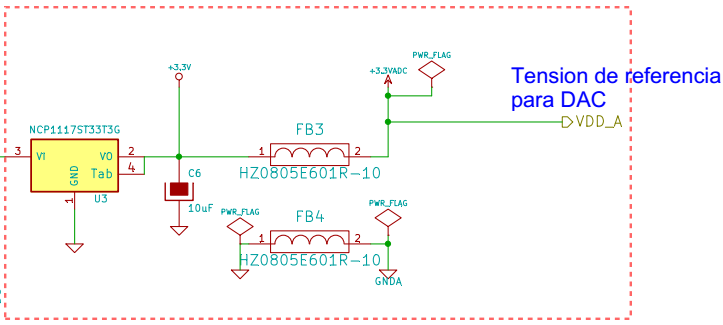
\includegraphics[width=8 cm]{figuras/f8.png}\\
\caption{Ilustración de tensión de referencia de DAC.}
\label{Fig26}
\end{figure}
\end{center}

\begin{enumerate}
\item[•]\underline{Estados}:
\begin{enumerate}
\item[•]Estado \textit{\textbf{LEO$\_$POTENCIOMETRO}}: Estado inicial, en el cual se determina la lectura analógica.
\item[•]Estado \textit{\textbf{SALIDA$\_$2}}: Estado en el cual se realiza una salida analógica igual a 2[V], en el caso que la lectura realizada sea superior a 2[V].
\item[•]Estado \textit{\textbf{SALIDA$\_$3}}: Estado en el cual se realiza una salida analógica igual a 3[V], en el caso que la lectura realizada sea superior a 4[V].
\end{enumerate}
\item[•]\underline{Eventos}:
\begin{enumerate}
\item[•]Evento \textit{\textbf{MAYOR$\_$2}}: Identifica si la lectura realizada sobre el ADC es superior a 2[V].
\item[•]Evento \textit{\textbf{MAYOR$\_$4}}: Identifica si la lectura realizada sobre el ADC es superior a 4[V].
\item[•]Evento \textit{\textbf{MENOR$\_$4}}: Identifica si la lectura realizada sobre el ADC es inferior a 4[V].
\item[•]Evento \textit{\textbf{NINGUNO}}: Identifica si la lectura realizada sobre el ADC es inferior a 2[V].
\end{enumerate}
\item[•]\underline{Acciones}
\begin{enumerate}
\item[•]Accion \textit{\textbf{APAGAR$\_$DAC}}: Establece una salida de 0 [V] sobre el terminal del DAC.
\item[•]Accion \textit{\textbf{DAC$\_$2}}: Establece una salida de 2 [V] sobre el terminal del DAC.
\item[•]Accion \textit{\textbf{DAC$\_$3}}: Establece una salida de 3 [V] sobre el terminal del DAC.
\end{enumerate}
\end{enumerate}

La Figura \ref{Fig28} ilustra el diagrama de estados que corresponde al ejemplo

\begin{center}
\begin{figure}[!h]
\centering
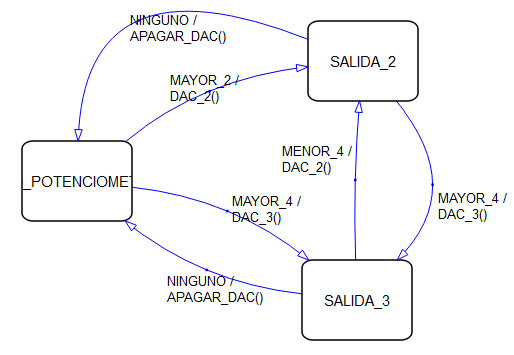
\includegraphics[width=6 cm]{figuras/f10.png}\\
\caption{Diagrama de estados de ejemplo N$^{\circ}$5}
\label{Fig28}
\end{figure}
\end{center}



\subsubsection{Implementacion de ejemplo N$^{\circ}$6: Comunicación Serial}
El siguiente ejemplo introduce al usuario en la utilización de comunicación serial, es necesario destacar que para la implementación del ejemplo se utiliza el programa \textit{Octoplus Terminal} para la visualización y simulación del envío y transmisión de datos a través del terminal conectado sobre el puerto USB.

El programa se encuentra disponible de forma gratuita en la dirección web \textit{http://octoplus-terminal.software.informer.com/download/}. La instalación de dicho programa es simple, sin embargo, es necesario destacar que durante dicho proceso, el usuario debe obviar la instalación de los drivers que provee dicho programa.

Si bien ofrece distintas herramientas para la programación de sistemas embebidos, este tutorial se centra en la utilización de dicho programa para el envío y la recepción de datos sobre el terminal perteneciente a la placa. Para ello, a continuación se realizará una serie de pasos para la utilización de \textit{Octoplus} junto con la placa:

\begin{enumerate}
\item[•]Suponiendo que el usuario ya se encuentran instalados los drivers para la placa, y las herramientas de depuración para la misma, luego de realizar la conexión entre la placa y la computadora a través de \textit{OpenOCD} (sobre la consola \textit{cygwin}), el usuario debe iniciar \textit{Octoplus}.
\item[•]A continuación se presenta una pantalla similar a la Figura \ref{Fig29}

\begin{center}
\begin{figure}[!h]
\centering
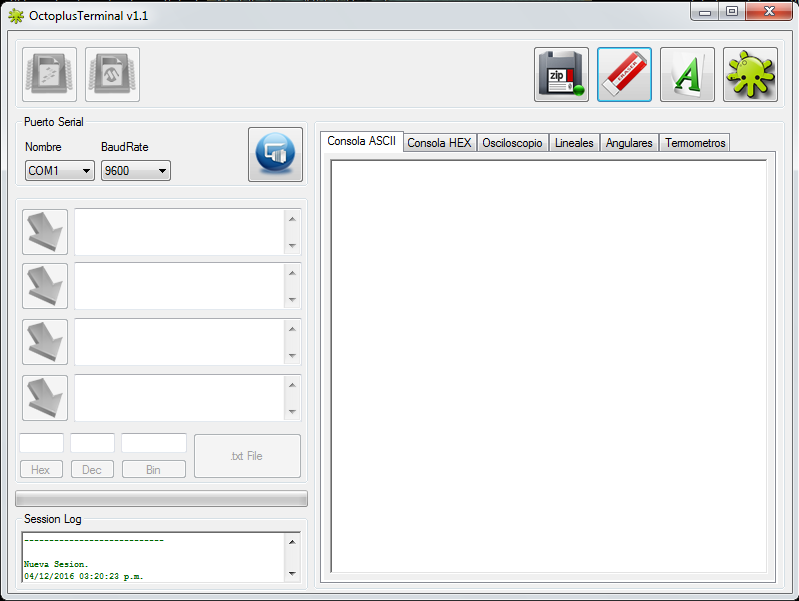
\includegraphics[width=6 cm]{figuras/f11.png}
\caption{Panel principal de \textit{Octoplus}}
\label{Fig29}
\end{figure}
\end{center}

\item[•]Sobre la sección \textit{Puerto Serial} debe identificarse sobre el menú desplegable \textit{Nombre}, el puerto COM asociado a la placa. La figura \ref{Fig30} ilustra dicho concepto

\begin{center}
\begin{figure}[!h]
\centering
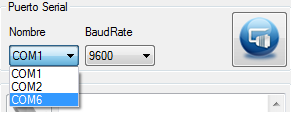
\includegraphics[width=4 cm]{figuras/f12.png}
\caption{Seleccion de puerto COM asociado a la placa}
\label{Fig30}
\end{figure}
\end{center}
\item[•]Debe tenerse en cuenta sobre la instrucción \textit{uartConfig()}, perteneciente a la librería \textit{sAPI}, deben asignarse dos parámetros de entrada, uno de ellos indica el módulo de la UART sobre la cual se desea trabajar, en este caso el parámetro es \textit{UART$\_$USB}. El segundo parámetro que debe asignarse a dicha instrucción es la velocidad de transmisión en baudios. El valor de la velocidad previamente configurada sobre el programa debe ser configurado sobre el menú desplegable \textit{BaudRate}, ubicado sobre el costado derecho del menú desplegable \textit{Nombre}.Por ejemplo, si la velocidad configurada es igual a 9600 baudios, entonces sobre dicho menú debe seleccionarse 9600, como lo ilustra la Figura \ref{Fig30}.
\item[•]Al realizar la depuración, el usuario debe seleccionar el boton \textit{Abrir/Cerrar puerto COM}, el cual se encuentra sobre la derecha del menú desplegable \textit{BaudRate},como lo ilustra la \ref{Fig29}.
\item[•]Para efectuar transmisiones sobre el puerto COM seleccionado, el usuario debe ingresar el dato sobre el cuadro de texto asociado al mismo y apretar el boton asociado a dicho cuadro.
\end{enumerate}

Es necesario mencionar que si existe un programa ya cargado previamente, también es posible utilizar \textit{Octoplus} de forma similar.

En este apartado se verá un código base para utilizar la UART del LPC4337 mediante las funciones que incluye la librería sAPI. Las funciones provistas por esta biblioteca son las encargadas de realizar los siguientes pasos básicos para poder utilizar la UART0 \cite{manuallpcuart}.

\begin{enumerate}
\item[•]Habilitar la alimentación del periférico.
\item[•]Habilitar el clock al periférico.
\item[•]Configurar la velocidad de transmisión.
\item[•]Habilitar las FIFO del transmisor y el receptor.
\item[•]Configurar la función de los pines para utilizarlo con la UART0.
\item[•]Habilitar la interrupción.
\end{enumerate}

\subsubsection{Implementacion de ejemplo N$^{\circ}$7:Comunicación Serial-Utilización Display LCD 16x2}
El siguiente ejemplo utiliza los leds incorporados en la placa, de forma tal que el numero de leds encendidos corresponda al caracter enviado. Por ejemplo, si se envía el caracter '3', entonces se encienden 3 leds.

En este ejemplo también se utiliza un display LCD 16x2. Para el manejo del mismo fue necesario utilizar una libreria no perteneciente a \textit{sAPI}, la cual fue diseñada por Matias Ferraro\cite{repositoriomatiasferraro}.

Para la implementación de la misma, se procede de forma similar a la realizada para el display de 7 segmentos, explicado anteriormente sobre la sección \ref{sec:ej2BM} .

Sobre la Figura \ref{Fig31} se ilustra el diagrama esquemático para el conexionado.

\begin{center}
\begin{figure}[!h]
\centering
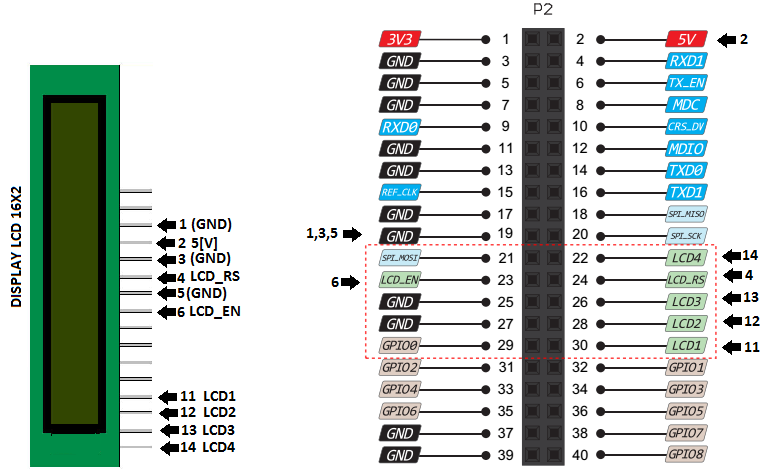
\includegraphics[width=8 cm]{figuras/f13.png}
\caption{Diagrama esquematico de conexion display LCD 16x2}
\label{Fig31}
\end{figure}
\end{center}

\section{Sistemas Operativos en Tiempo Real}
Un Sistema Operativo es un conjunto de programas que ayuda al programador de aplicaciones a gestionar recursos de hardware disponible, entre ellos el tiempo del procesador y la memoria (citar).
Una parte del OS se encarga de asignar el tiempo de ejecución a todos los programas que tiene cargados en base a un juego de reglas conocido de antemano. A dichos subprogramas se los denomina Tareas.

Con esto se logra aparentar que múltiples programas se están ejecutando simultaneamente, sin embargo solo pueden hacerlo de uno a la vez.

El encargado de realizar esta gestión es un componente del sistema operativo denominado Scheduler o Programador de Tareas. La función de éste es determinar que tarea debe estar en ejecución a cada momento.

Ante la ocurrencia de ciertos eventos el Scheduler revisa si la tarea en ejecución debe reemplazarse por alguna otra tarea. A este reemplazo se lo denomina cambio de contexto de ejecución.

Debido a que el OS debe guardar el contexto completo de la tarea actual, y reemplazarlo por la tarea reentrante, debe reservarse un bloque de la memoria de datos para cada tarea. Lo cual limita el número de tareas que pueden ejecutarse de forma simultánea.Los cambios de contexto que se realizan cuando se reemplaza una tarea por otra no agregan trabajo al programador, de modo que al retornar a dicha tarea, el programador no observa ningún sintoma de haberla pausado alguna vez.

Un RTOS (sigla de \textit{Real Time Operating System}) realiza la misma función que un OS común, sin embargo agrega herramientas para que los programas de aplicación puedan cumplir compromisos temporales definidos por el programador. De modo que se encuentran diseñados para la administración de varias tareas simultáneas con plazos de tiempo estrictos.

El RTOS ofrece funcionalidad para asegurar que una vez ocurrido un evento, la respuesta ocurra en un tiempo acotado.Es necesario destacar que esto no lo hace por si solo sino que brinda al programador herramientas para implemetarlo de forma mas simple.

\subsection{Tareas}\label{sec:tareas}
El bloque básico de software escrito sobre un RTOS es la Tarea, sobre la mayoria de las RTOS que se ofrecen en el mercado, una Tarea es una simple subrutina\cite{librodertoseningles}.

Una Tarea provee un contexto en el cual se ejecuten las funciones.Mientras que el Scheduler organiza la secuencia de ejecución de las tareas(referencia os223).
En algún punto del programa se produce el llamado a alguna función que produzca la ejecución de dicha tarea(referencia libro).

En el sistema operativo OSEK las Tareas deben ser definidas en la configuración, de manera que no es posible crear Tareas de forma dinámica (a diferencia de los Sistemas Operativos de escritorio). En el momento de la compilación se genera el código del sistema operativo y se definen la cantidad de Tareas y sus características. Además deben utilizarse macros para las definiciones y las funciones (a dichas funciones se las suele denominar Servicios del Sistema ) que ofrece este Sistema Operativo, para ello, debe incluirse sobre el programa, \textit{os.h}.

Este sistema operativo ofrece dos conceptos distintos de Tareas:
\begin{enumerate}
\item[•]Tareas del tipo \emph{BASIC}:Este tipo de Tareas solamente libera al procesador en los siguientes casos:
\begin{enumerate}
\item[1]Cuando terminan.
\item[2]Cuando son interrumpidas por acción del Scheduler, al realizar la activación de una Tarea que posea mayor prioridad (caracteristica propia de los Sistemas Operativos del tipo \textit{preemptive}).
\item[3]Ocurre una interrupción que causa que el procesador acuda a una subrutina de atencion de interrupción.
\end{enumerate}
\item[•]Tareas del tipo \emph{EXTENDED}: Se distinguen de las Tareas extendidas por el hecho de que pueden utilizar una funcion propia de este OS, denominado \textit{WaitEvent()}. Este tipo de Tareas permite liberar el procesador y ser relevado hacia Tareas de menor prioridad, sin la necesidad de que finalize la Tarea que se encuentra esperando.
%DECIDIR SI ESTO VA O NO..DADO QUE NO ENCUENTRO DE DONDE LO SAQUE%
La ventaja de las Tareas extendidas es que pueden manejar coherentemente una Tarea sin importar que eventos de sincronización se encuentren activos%%
\subsubsection{Modelo de Tareas Básicas}
El modelo de las Tareas Basicas es similar al de las Tareas Extendidas, excepto que éstas no contienen un estado \textit{Waiting}. A continuación se realiza una breve descripción de los estados definidos sobre este tipo de Tareas.
\begin{enumerate}
\item[•]\textbf{\emph{Running}}:En este estado, la CPU es asignada a la Tarea, de modo que se ejecutan sus instrucciones. Solamente una sola Tarea (sin importar de que tipo sea) puede estar en este estado, en un instante determinado; mientras las demás Tareas pueden adoptar otros estados.
\item[•]\textbf{\emph{Ready}}: Se cumplieron todos los pre-requisitos para que la Tarea adquiera el estado \textit{Running}.El \textit{Scheduler} decide cuál Tarea en estado \textit{Ready} será desplazada al estado \textit{Running}.
\item[•]\textbf{\emph{Suspended}}: En este estado, la Tarea se encuentra en estado pasivo y puede ser activada.
\end{enumerate}
La Figura \ref{Fig32} ilustra los conceptos explicados previamente.
\begin{center}
\begin{figure}[!h]
\centering
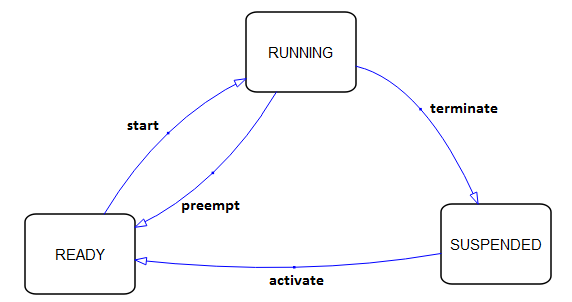
\includegraphics[width=8 cm]{figuras/f14.png}
\caption{Modelo de las Tareas del tipo \textit{BASIC}}
\label{Fig32}
\end{figure}
\end{center}
\end{enumerate}

El Cuadro \ref{Tab3} explica los diferentes eventos que provocan las transiciones entre los estados. 

\begin{table}[h]
\begin{center}
\resizebox{18cm}{!}{
\begin{tabular}{|l|l|l|l|}
\hline\hline
\textbf{{\Large Transicion}} & \textbf{{\Large Estado Actual}} & \textbf{{\Large Nuevo Estado}} & \textbf{{\Large Descripcion}}\\ \hline
\textbf{{\Large activate}}&{\Large suspended}&{\Large ready}&{\Large Una nueva tarea se asigna al estado} \textit{{\Large Ready}} {\Large por el OS}.\\ \hline
\textbf{{\Large start}}&{\Large ready}&{\Large running}&{\Large Una Tarea en estado} \textit{{\Large Ready}} {\Large es seleccionada por el} \textit{{\Large Scheduler}} {\Large para ser ejecutada}\\ \hline
\textbf{{\Large preempt}}&{\Large running}&{\Large ready}&{\Large El} \textit{{\Large Scheduler}} {\Large decide empezar otra Tarea. La Tarea que estaba en estado} \textit{{\Large Running}} {\Large se establece en estado} \textit{{\Large Ready}}.\\ \hline
\textbf{{\Large terminate}}&{\Large running}&{\Large suspended}&{\Large La tarea en estado} \textit{{\Large Running}} {\Large se establece en estado} \textit{{\Large Suspended}} {\Large gracias a la acción de algún servicio del sistema}.\\ \hline
\end{tabular}
}
\caption{Tabla de transiciones de las Tareas del tipo \textit{Basic}.}
\label{Tab3}
\end{center}
\end{table}

\subsubsection{Modelo de Tareas Extendidas}
El modelo de las Tareas Extendidas posee cuatro estados:
\begin{enumerate}
\item[•]\emph{\textbf{Running}}: En dicho estado, la CPU es asignada a la Tarea, de modo que se ejecuten las instrucciones que contiene la misma. Solamente una Tarea puede encontrarse en dicho estado en un instante determinado, mientras las otras Tareas pueden adoptar los demas estados.
\item[•]\emph{\textbf{Ready}}: Se cumplieron todos los pre-requisitos necesarios para la transición al estado \textit{Running}. El \textit{Scheduler} decide cuál de las tareas en estado \textit{Ready} será ejecutada a continuación.
\item[•]\emph{\textbf{Waiting}}:La ejecución de una Tarea no puede continuar debido a que debe $"$esperar$"$ a que un evento ocurra.
\item[•]\emph{\textbf{Suspended}}: La Tarea se encuentra en modo pasivo hasta que se active.
\end{enumerate}

La Figura \ref{Fig33} ilustra los conceptos explicados previamente.
\begin{center}
\begin{figure}[!h]
\centering
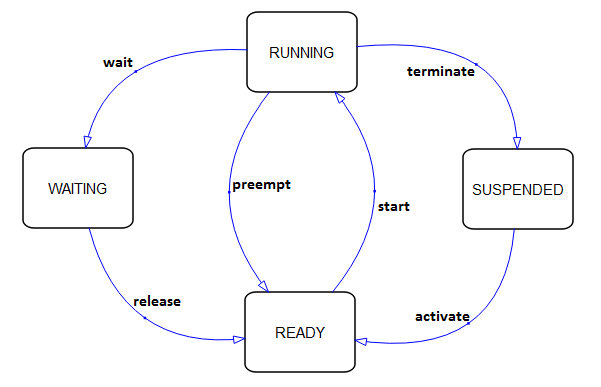
\includegraphics[width=8 cm]{figuras/f15.png}
\caption{Modelo de las Tareas del tipo \textit{EXTENDED}}
\label{Fig33}
\end{figure}
\end{center}

El Cuadro \ref{Tab4} explica los diferentes eventos que provocan las transiciones entre los estados. 

\begin{table}[h]
\begin{center}
\resizebox{18cm}{!}{
\begin{tabular}{|l|l|l|l|}
\hline\hline
\textbf{{\LARGE Transicion}} & \textbf{{\LARGE Estado Actual}} & \textbf{{\LARGE Nuevo Estado}} & \textbf{{\LARGE Descripcion}}\\ \hline
\textbf{{\LARGE activate}}&{\LARGE suspended}&{\LARGE ready}&{\LARGE Una nueva tarea se asigna al estado }\textit{{\LARGE Ready}} {\LARGE por el OS}.\\ \hline
\textbf{{\Large start}}&{\Large ready}&{\Large running}&{\Large Una Tarea en estado} \textit{{\Large Ready}} {\LARGE es seleccionada por el} \textit{{\Large Scheduler}} {\Large para ser ejecutada}\\ \hline
\textbf{{\Large wait}}&{\Large running}&{\Large waiting}&{\Large La tarea se establece en estado} \textit{{\Large Waiting}} {\Large debido a la accion de un Servicio del Sistema.} \\ \hline
\textbf{{\Large release}}&{\Large waiting}&{\Large ready}&{\Large Al menos ocurrió un evento que esperaba la Tarea}\\ \hline
\textbf{{\Large preempt}}&{\Large running}&{\Large ready}&{\Large El} \textit{{\Large Scheduler}}{\Large decide iniciar otra Tarea. La Tarea que se encontraba en estado} \textit{{\Large Running}},{\Large  se establece en estado} \textit{{\Large Ready}}.\\ \hline
\textbf{{\Large terminate}}&{\Large runnning}&{\Large suspended}&{\Large La Tarea en estado} \textit{{\Large Running}} {\Large se establece al estado} \textit{{\Large Suspended}} {\Large gracias a un Servicio del Sistema}.
\end{tabular}
}
\caption{Transiciones de las Tareas del tipo \textit{Extended}.}
\label{Tab4}
\end{center}
\end{table}

\underline{Activación de Tareas}: 

La activación de una Tarea es realizada mediante el Servicio del Sistema \textit{ActivateTask} o por \textit{ChainTask}. Luego de la activación de una Tarea, ésta se encuentra lista para ejecutarse desde su primer instrucción. En el caso que se produzcan múltiples activaciones de una Tarea del tipo \textit{BASIC}, el Sistema Operativo OSEK almacena estas activaciones paralelas, siempre y cuando se haya definido sobre éste, una clase de conformidad.

\underline{Finalización de las tareas}:

En el Sistema Operativo OSEK, una Tarea solo puede finalizarse por acción propia, mediante el Servicio del Sistema \textit{TerminateTask}. Cabe destacar que el Servicio del Sistema \textit{ChainTask} provee una forma de realizar la activación de una Tarea determinada, justo después de la finalización de la Tarea que se encuentra corriendo.

Esta estrictamente prohibido realizar una Tarea que no finalize con alguno de estos dos Servicios del Sistema, dado que puede ocasionar un comportamiento indefinido.

\underline{Prioridad de las tareas}:

La asignación de prioridades sobre las Tareas se realiza a través de la definición de números enteros desde 0 hasta 255. Mientras mayor es el valor del numero, mayor será la prioridad.Una Tarea que se encuentra corriendo, no puede ser interrumpida por una de menor o igual prioridad.
\subsection{Scheduler}\label{sec:scheduler}
El algoritmo del Scheduler puede ser visto fundamentalmente como un coordinador de Tareas con las prioridades ya establecidas, en el cual se define un número máximo de activaciones de las mismas. El sistema operativo OSEK define tres politicas de \textit{Scheduling}, las cuales se mencionan a continuación.

\underline{\textit{Scheduling Full Preemptive}}:

Esta politica de \textit{Scheduling} implica que una Tarea que se encuentra en el estado \textit{Running} puede ser interrupida sobre cualquier instrucción, como consecuencia de la ocurrencia de alguna condición o evento; que ya se encuentre definido previamente sobre el OS. \textit{Full Preemptive Scheduling} determinará que una Tarea en el estado \textit{Running} sea establecido en el estado \textit{Ready}, tan pronto como una Tarea de mayor prioridad se establezca en estado \textit{\textit{Ready}}.

El contexto de la Tarea será almacenado de forma que la Tarea que fue interrumpida pueda continuar sobre la instancia en donde fue interrumpida.

\underline{\textit{Scheduling Non Preemptive}}:

Cuando el cambio de Tareas solo se produce mediante la ejecución de algún Servicio del Sistema (explicitados en los puntos de \textit{Scheduling}).


\underline{Puntos de \textit{Scheduling}}:

\begin{enumerate}
\item[•]Puntos de \textit{Scheduling} en una tarea \textit{NON-PREEMPTIVE}
\begin{enumerate}
\item[•]Al llamar a la interfase \textit{Schedule} cuando retorna E$\_$OK.
\end{enumerate}
\item[•]Puntos de \textit{Scheduling} en una tarea \textit{PREEMPTIVE}
\begin{enumerate}
\item[•]Al finalizar un llamado a la interfase \textit{ActivateTask} que retorna E$\_$OK.
\item[•]Al finalizar un llamado a la interfase \textit{ChainTask} que no retorna.
\item[•]Al finalizar un llamado a la interfase \textit{TerminateTask} que no retorna.
\item[•]Al finalizar un llamado a la interfase \textit{ReleaseResource} que retorna E$\_$OK.
\item[•]Al finalizar un llamado a la interfase \textit{SetEvent} que no retorna.
\item[•]Al expirar una alarma que activa una tarea.
\item[•]Al terminar la ejecución de una ISR de categoría 2
\end{enumerate}
\end{enumerate} 

\subsection{Modos de Aplicación}
Los Modos de Aplicación son designados sobre un Sistema Operativo OSEK, para trabajar sobre diferentes modos de operación. El número mínimo de modos de aplicación que puede soportar este Sistema Operativo es igual a 1. Un ejemplo que puede ilustrarse es la definición de dos modos de operación, uno para la operación normal del programa, y otro para la finalización de la misma.

\subsection{Eventos}

Los eventos son objetos manejados por el OS. Es posible considerarla de forma abstracta como un bit o un flag, que puede ser enmascarado.Dichos eventos pueden ser seteados o restablecidos utilizando Servicios del Sistema. Es importante destacar que solamente las Tareas del tipo \textit{EXTENDED} pueden utilizar esta herramienta para permitir la sincronización de las mismas. El Servicio del Sistema \textit{WaitEvent} permite esperar al suceso del evento, para poder realizar las instrucciones que contenga dicha Tarea.

Las Tareas del tipo \textit{EXTENDED} típicamente poseen su propio \textit{stack} o pila que registra el suceso de dicho evento. Sin embargo, es muy importante destacar que este tipo de Tareas solo pueden ser activadas una sola vez.

Un evento individual es identificado por el propietario de dicho evento, y por su nombre (denominado Máscara según la especificación).Cuando una Tarea de tipo \textit{EXTENDED} es activada, los eventos asignados a la misma son establecidos a 0 por el OS. El significado de un evento es definido por la aplicación; por ejempo, puede significar que ha expirado un \textit{Timer}, puede significar que se encuentra disponible un recurso, puede significar la recepción de un mensaje, etc.

Existen varias opciones disponibles para manipular los eventos, tanto para las Tareas que son propietarias de dicho Evento, como de las demás Tareas que no son propietarias del Evento, las cuales no necesariamente deben ser Tareas del tipo \textit{EXTENDED}.

Todas las Tareas e Interrupciones del tipo \textit{ISR2} pueden indicar el suceso de un Evento e informarlo a la Tarea propietaria del evento (del tipo \textit{EXTENDED}) siempre y cuando no se encuentre en estado \textit{SUSPENDED}.Sin embargo, solamente la Tarea propietaria de dicho Evento puede restablecer el flag del Evento.

Debe destacarse que cuando una Tarea tipo \textit{EXTENDED}, se encuentra en estado \textit{Waiting}, se establece en el estado \textit{Ready} si al menos ocurre uno de los Eventos que dicha Tarea estaba esperando. Si una Tarea tipo \textit{EXTENDED} se encuentra ejecutándose y trata de esperar un Evento que ya haya ocurrido, dicha Tarea se mantiene en el estado \textit{Running}.

\subsection{Clases de Conformidad}
Con la finalidad de permitir que OSEK-OS pueda ser utilizado en una gran variedad de sistemas con diferentes capacidades y demandas (por ejemplo memoria, capacidad de procesamiento, etc.) es que OSEK-OS define 4 clases de conformidad (CC).

Las diferentes clases existen para poder comparar entre sistemas, agrupar las interfaces según la clase de conformidad y facilitar la certificación de conformidad.

Las clases de conformidad se determinan según los siguientes atributos: 

\begin{enumerate}
\item[•]Múltiple activaciónde tareas básicas.
\item[•]Tipos de tareas aceptadas: básicasy extendidas.
\item[•]Cantidad de tareas por prioridad.
\end{enumerate}

De esta forma se definen las siguientes clases de conformidad:
\begin{enumerate}
\item[•]BCC1: que soporta únicamente tareas  básicas con máximo una activación por tarea, y todas las tareas con prioridad diferente.
\item[•]BCC2: como  BCC1 pero con más de una tarea por prioridad y las tareas soportan más de una activación.
\item[•]ECC1: como BCC1 pero con tareas extendidas.
\item[•]ECC2: como  ECC1 pero con más de una tarea por prioridad y las tareas soportan más de una activación.
\end{enumerate}
El OSEK-OS de la CIAA soporta todas las conformidades. Dependiendo de esta configuración el sistema decidirá si se implementa una clase BCC1 o ECC2. Por lo que para el usuario final del CIAA-Firmware es prácticamente irrelevante conocer las clases. El Firmware decide automáticamente y configura la clase de conformidad correcta según los requerimientos del usuario.La Figura 37 ilustra los conceptos presentados anteriormente.


\begin{figure}[!h]
\centering
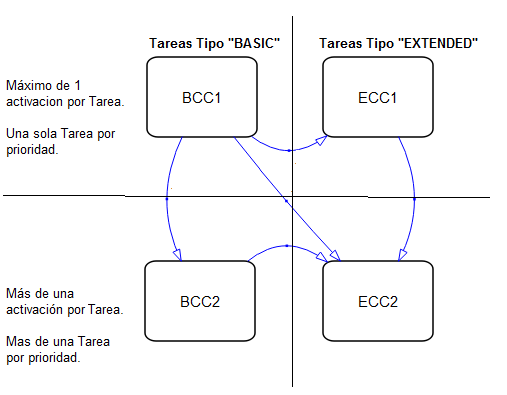
\includegraphics[width=8 cm]{figuras/f17.png}
\caption{Clases de Conformidad.}
\label{Fig34}
\end{figure}

\subsection{Configuración y Generación}\label{sec:generacionoil}
Al ser OSEK-OS un sistema estático es necesario configurarlo. La cantidad de tareas, que prioridad tienen las mismas, el tamaño de pila que utilizan, etc. Para ello OSEK-VDX definió otro estándar llamado OSEK Implementation Language comúnmente llamado "OIL".

OIL es un lenguaje textual con una sintaxis similar al lenguaje C donde se indican las características del sistema operativo como ser: tareas, prioridades, pila, interrupciones etc.El siguiente ejemplo ilustra al usuario sobre la generación de dicho archivo.

\subsubsection{Implementacion de ejemplo N$^{\circ}$1: Tareas en OSEK}
Este ejemplo utiliza los leds de la placa y un Display 7 Segmentos, para implementar un contador de numeros decimales, a través de una sola Tarea del tipo \textit{BASIC}.

En primer lugar es necesario generar el archivo OIL para configurar el Sistema Operativo OSEK. A través del \textit{Bloc de Notas} o a través de cualquier editor de texto, debe iniciar la configuración a través de la sintaxis \textit{OSEK OSEK} y sobre los simbolos { y } ,se determinarán los restantes aspectos que tendra el OS.La Figura 38 ilustra lo mencionado anteriormente.


\begin{figure}[!h]
\centering
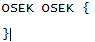
\includegraphics[width=5 cm]{figuras/f18.png}
\caption{Inicio de Archivo de Configuración.}
\label{Fig35}
\end{figure}

Luego debe definirse mediante la sintaxis \textit{OS}, el nombre del sistema operativo (el cual es arbitrario, dado que se ha especificado en la instruccion anterior que se implementa un sistema operativo OSEK), la Figura ilustra el concepto explicado anteriormente.

\begin{figure}[!h]
\centering
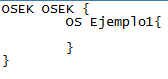
\includegraphics[width=5 cm]{figuras/f19.png}
\caption{Archivo de Configuración:Comienzo de especificación}
\label{Fig36}
\end{figure}

A continuación debe definirse las siguientes configuraciones para el OS del ejemplo:

\begin{enumerate}
\item[•]El nivel de chequeo de errores que se pueden producir. Existen dos niveles que pueden determinarse:
\begin{enumerate}
\item[•]\textit{STANDARD}: Implica un chequeo mínimo de errores, se encuentra pensado para unidades de producción en serie.La instrucción utilizada es \textit{OS = STANDARD}. 
\item[•]\textit{EXTENDED}: Implica un chequeo máximo de errores y \textit{debug hooks}.La instrucción utilizada es \textit{OS = EXTENDED}.
\end{enumerate}
\item[•]Funciones implementadas por el usuario que el OS llamará en circunstancias específicas, tales como:
\begin{enumerate}
\item[•]\textit{Startuphook}: es  llamada  durante  la  inicialización  del  sistema  operativo,  antes  de  ser completada. En caso de utilizarla se debe escribir la instrucción \textit{STARTUPHOOK = TRUE}; en caso contrario se debe asignar \textit{FALSE}.
\item[•]\textit{Shutdownhook}: es llamada al finalizar el apagado del sistema operativo.En caso de utilizarla se debe escribir la instrucción \textit{SHUTDOWNHOOK = TRUE}; en caso contrario se debe asignar \textit{FALSE}.
\item[•]\textit{Pretaskhook}: es llamada antes de proceder a ejecutar una tarea.En caso de utilizarla se debe escribir la instrucción \textit{PRETASKHOOK = TRUE}; en caso contrario se debe asignar \textit{FALSE}.
\item[•]\textit{Posttaskhook}:es llamada al finalizar la ejecución de una tarea.En caso de utilizarla se debe escribir la instrucción \textit{POSTTASKHOOK = TRUE}; en caso contrario se debe asignar \textit{FALSE}.
\item[•]\textit{Errorhook}:es llamada en caso de que alguna de las interfaces del sistema operativo retorne un valor distinto a E$\_$OK.En caso de utilizarla se debe escribir la instrucción \textit{ERRORHOOK = TRUE}; en caso contrario se debe asignar \textit{FALSE}.
\end{enumerate}
\item[•]Uso del \textit{Scheduler} como recurso.
\item[•]Uso del mapa de memoria.
\end{enumerate}
La Figura  ilustra un OS configurado de forma que el nivel de chequeo de errores sea el mínimo, y solamente se defina una función para en caso de un error producido en el OS.

\begin{figure}[!h]
\centering
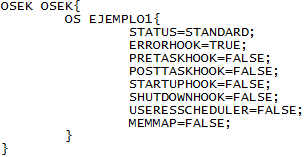
\includegraphics[width=5 cm]{figuras/f20.png}
\caption{Archivo de Configuración:Ejemplo de especificación de OS}
\label{Fig37}
\end{figure}

\ref{Fig37}

\begin{thebibliography}{}
\bibitem{origeneduciaa} {\footnotesize http://proyecto-ciaa.com.ar/devwiki/doku.php?id=proyecto:origen$\_$ciaa}

Fecha: 15/10/16 10:55 am.
\bibitem{descripcionenhojadatos}\textit{UM10503
LPC43xx/LPC43Sxx ARM Cortex-M4/M0 multi-core
microcontroller} Pags: 12-16.
\bibitem{diagramaenbloquesdeplaca} {\footnotesize http://proyecto-ciaa.com.ar/devwiki/doku.php?id=desarrollo:edu-ciaa:edu-ciaa-nxp}

Fecha: 15/10/16 10:55 am.
\bibitem{descripcionopenocd}{\footnotesize http://proyecto-ciaa.com.ar/devwiki/doku.php?id=desarrollo:firmware:instalacion$\_$sw$\&$s[]=puente}\

Fecha: 15/10/16 11:00 am.
\bibitem{parametrosdelmakefile} {\footnotesize http://proyecto-ciaa.com.ar/devwiki/doku.php?id=docu:fw:bm:make$\&$s[]=makefile}

Fecha: 15/10/16 11:00 am.
\bibitem{estructuradedirectorios} {\footnotesize http://proyecto-ciaa.com.ar/devwiki/doku.php?id=docu:fw:bm:estructura$\&$s[]=estructura$\&$s[]=de$\&$s[]=directorios} Fecha: 15/10/16 11:00 am.
\bibitem{sapi}\textit{sAPI:Introducción}

Documento existente sobre el repositorio ubicado en \textit{Github}.

Dirección web: https://github.com/epernia/sAPI

\bibitem{librodertoseningles}\textit{"An Embedded Software Primer"} Primera Edición Autor: David E. Simon Editorial: Pearson Education. Pags: 138-139.

\bibitem{manuallpcuart} \textit{UM10503 LPC43xx/LPC43Sxx ARM Cortex-M4/M0 multi-core microcontroller} Capítulo 40.

\bibitem{repositoriomatiasferraro}{\footnotesize https://github.com/MatiasFerraro/CIAA-MatiasFerraro} 

Fecha: 30/10/16 16:00 pm.
\end{thebibliography}

\end{document}
